%%%%%%%%%%%%%%%%%%%%%%
% Signal selection   %
%%%%%%%%%%%%%%%%%%%%%%

The signal region selection aims for a good discrimation between possible signals and the SM
backgrounds. As mentioned before, the signals we target with this search have $\cPqb$ tagged jets
and boosted $\W$ bosons in the final state. Therefore, we require, on top of the baseline
selection, the presence of at least one CSV medium $\cPqb$ tagged jet, and at least one $\W$ boson
tagged jet. AK5 jets are used for $\cPqb$ tagging, whereas for $\W$ tagging we use the CA8 jets, as
explained in Section~\ref{sec:boost_wtag}. 
Additionally, we only consider fully-hadronic events and thus select only those events with no
loose electrons or muons, and no isolated tracks. 
These selection criteria already reduce the background substantially, but it is not yet sufficient
to get a good signal separation. We need an additional handle on the QCD multijet production,
which is the dominant background at this stage. 

Missing transverse energy, \ETm, in multijet events is largely due to jet mismeasurements,
rather than the escape of weakly interacting particles, such as neutrinos or the neutralinos in
signal events. The \ETm vector will, therefore, often be aligned with one of the jets. 
Based on this we can expect that $\Delta\phi_{min}$, the minimum of the angles between \VEtmiss and
the transverse momentum of the leading three jets, will be a good discriminant between multijet
events and events with real \ETm.
\begin{equation}
 \Delta\phi_{min} = \min_{i=1,2,3}{\Delta\phi(\VEtmiss, \ptvec^{\,i})},
\end{equation}
where $i$ runs over the three AK5 jets. We require $\Delta\phi_{min} > 0.5$ to suppress multijet
events. 

A summary of the signal selection is presented in Table~\ref{tab:boost_selection_summary}.
Figure~\ref{fig:boost_signal_dataMC} shows the simulated distributions in the signal region for the
$\mr$ and $\rsq$ variables. The number of events in simulation and data, and the background
composition in percent, are reported in Table~\ref{tab:cutflow} and
Table~\ref{tab:BG_comp_percent}, respectively. 
The signal region is $t\bar{t}$ dominated, with additional contributions from $\W(\rightarrow
\ell\nu)+$jets and multijet processes.

\begin{figure}[htbp]
\centering
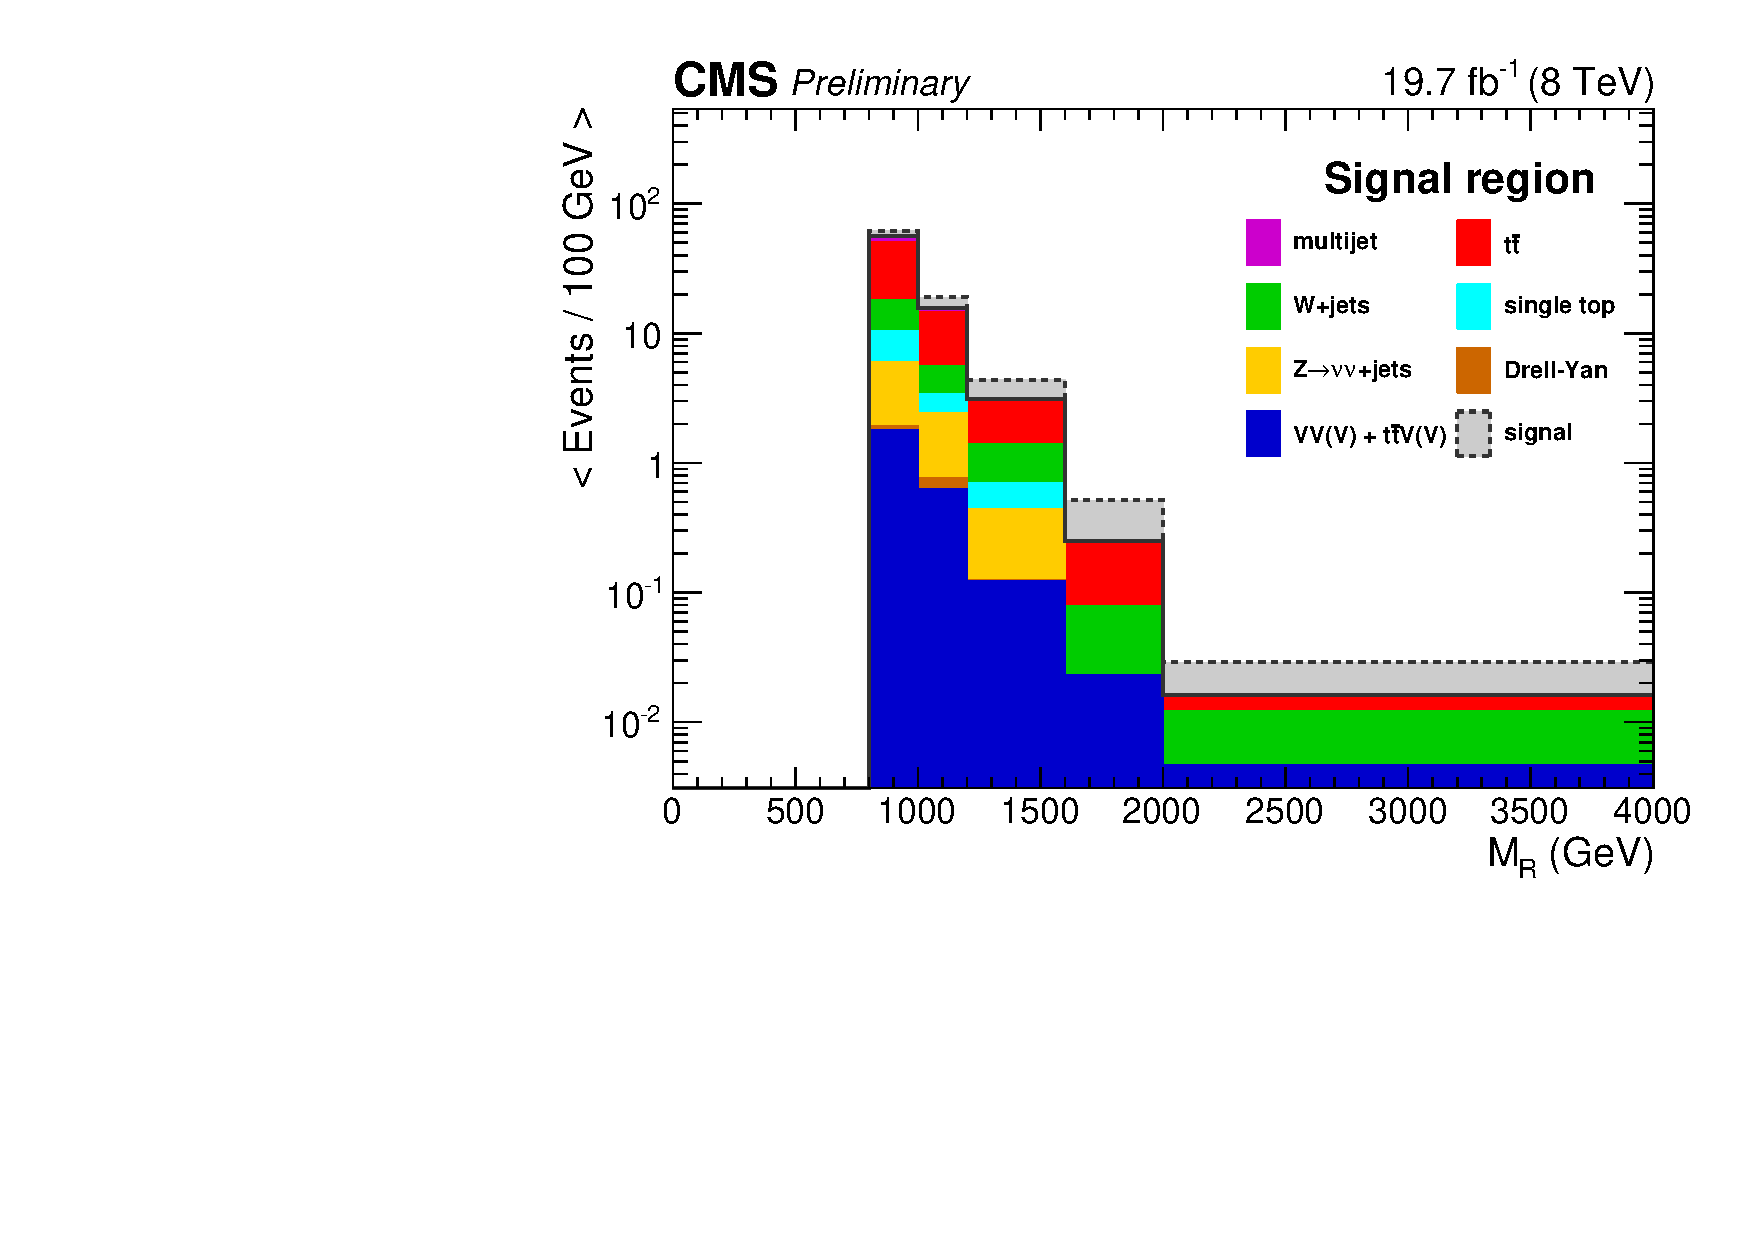
\includegraphics[width=0.48\textwidth]
{figures/razor_selection/DataMC_MR_g1Mbg1W0Ll_mdPhig0p5_width_nodata}
~
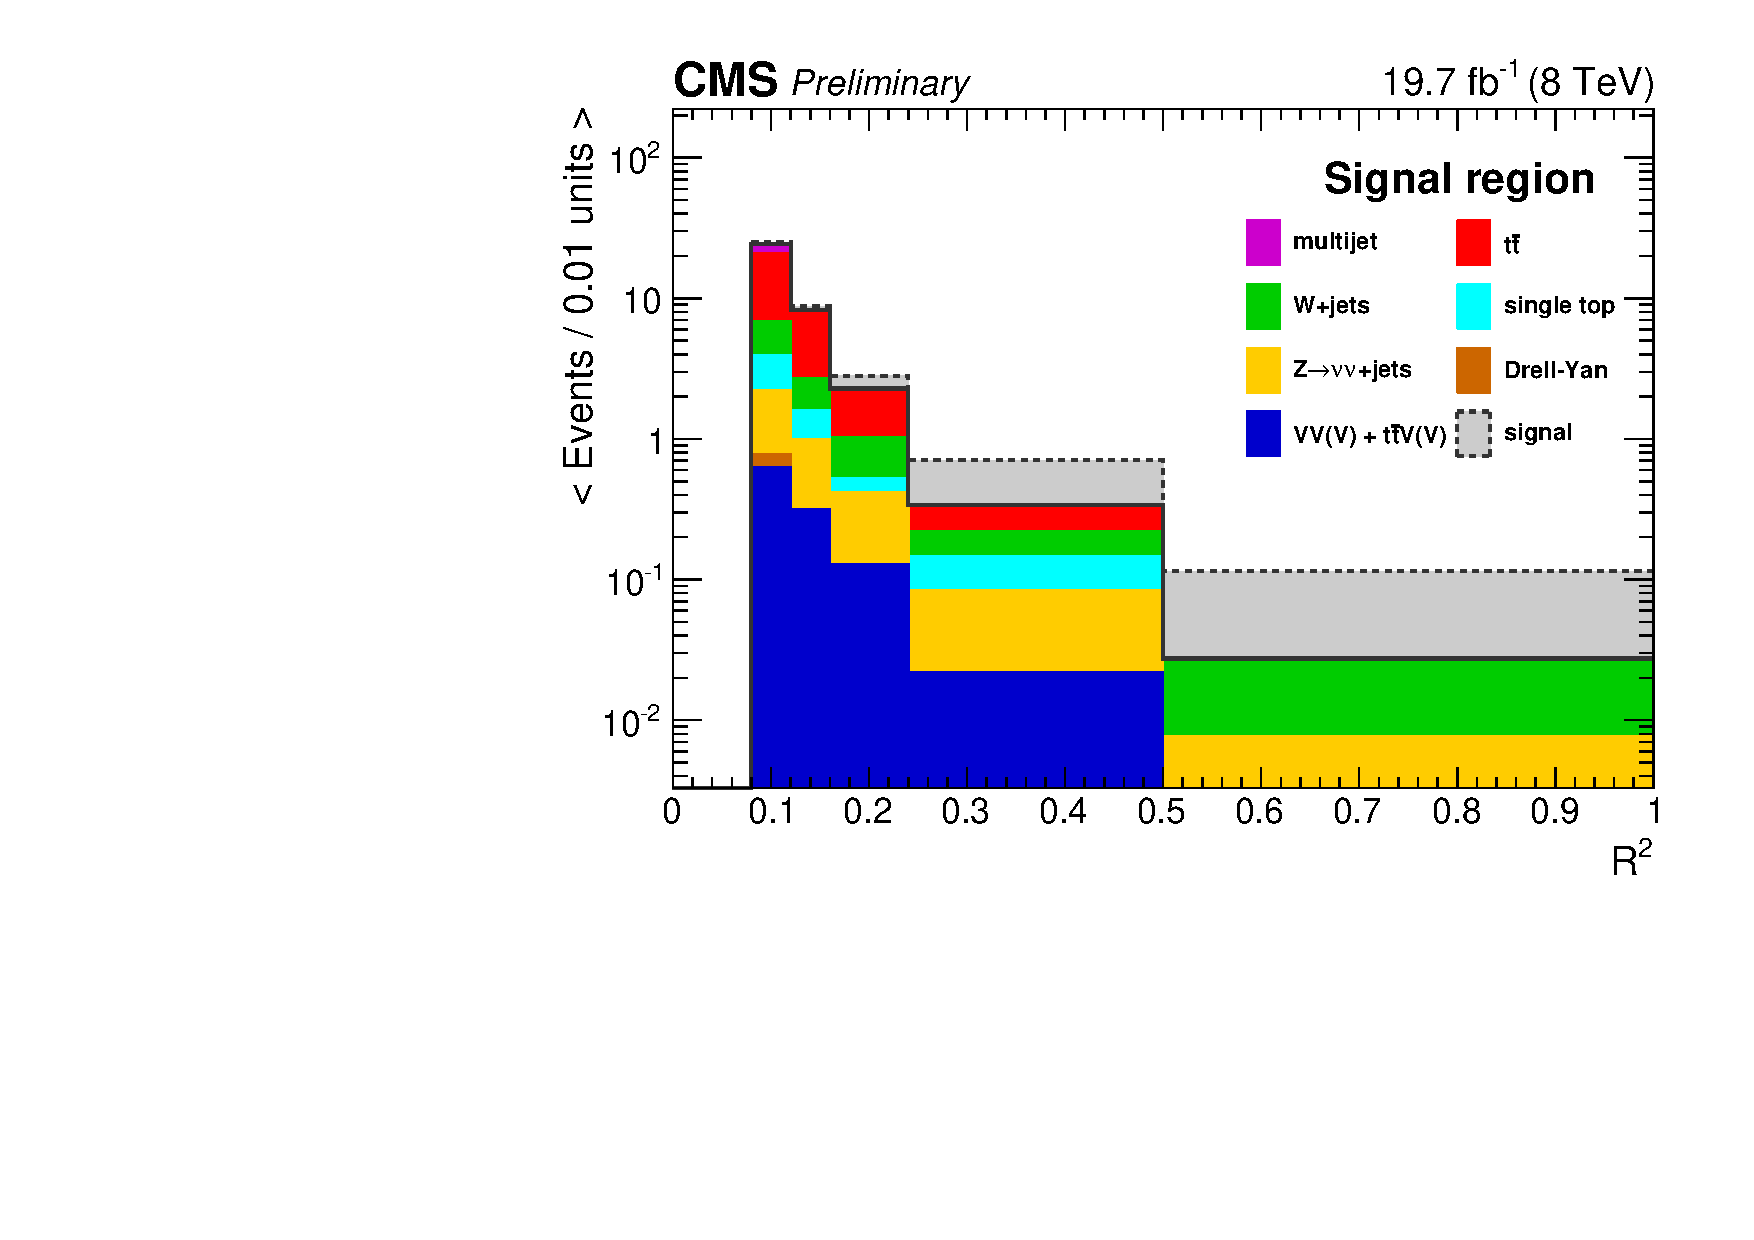
\includegraphics[width=0.48\textwidth]
{figures/razor_selection/DataMC_R2_g1Mbg1W0Ll_mdPhig0p5_width_nodata}
\caption{Simulated $\mr$ (left) and $\rsq$ (right) distributions in the signal region. An example
signal point, corresponding to the {\it T1ttcc} mass point with $m_{\tilde{g}}
\,{=}\, 1\TeV$, $m_{\stopone} \,{=}\, 325\GeV$ and $m_{\lsp} \,{=}\, 300\GeV$, is
stacked on top of the background processes. The bin entries are normalized proportional to the bin
width.  
\label{fig:boost_signal_dataMC}}
\end{figure}

% \begin{figure}[htbp]
% \centering
%  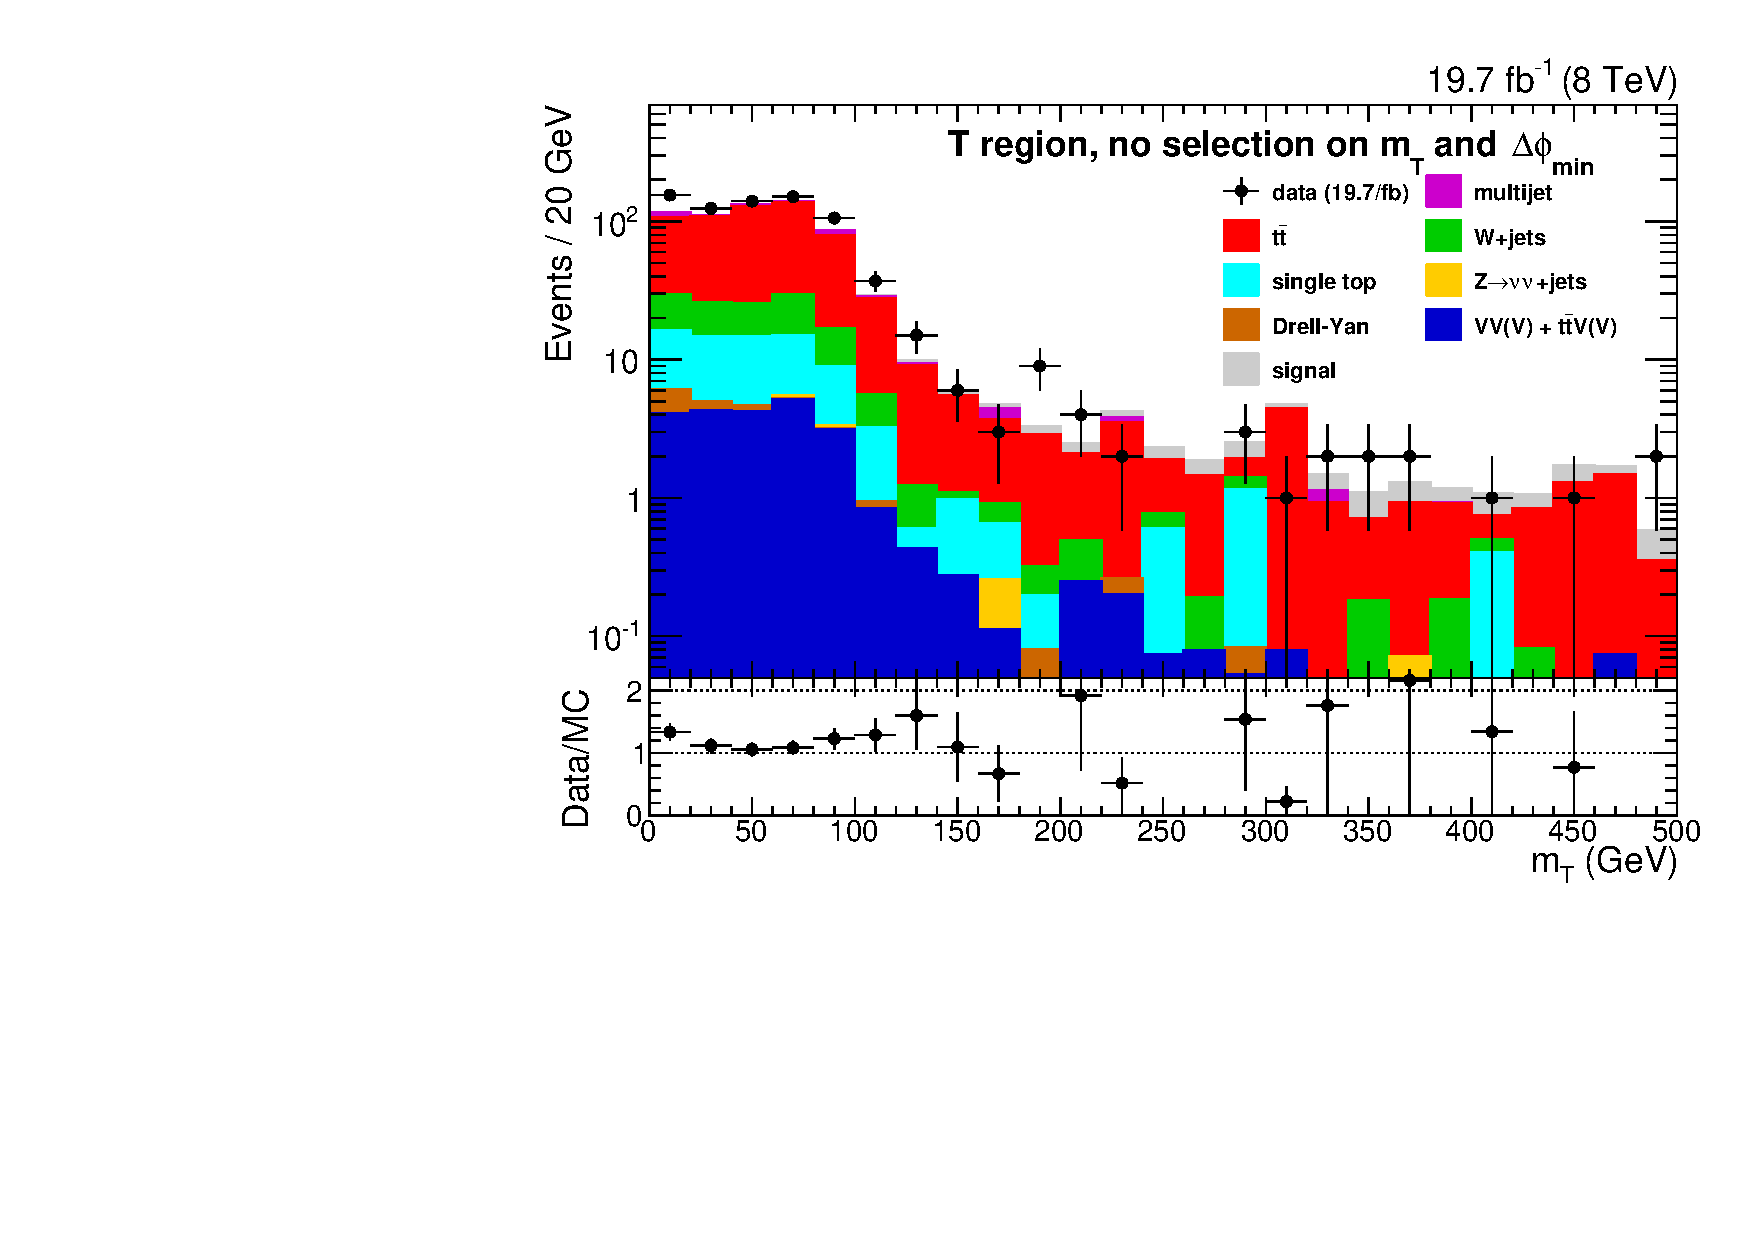
\includegraphics[width=0.49\textwidth]{figures/DataMC/DataMC_mT_g1Mbg1W1Ll_rebin}
%  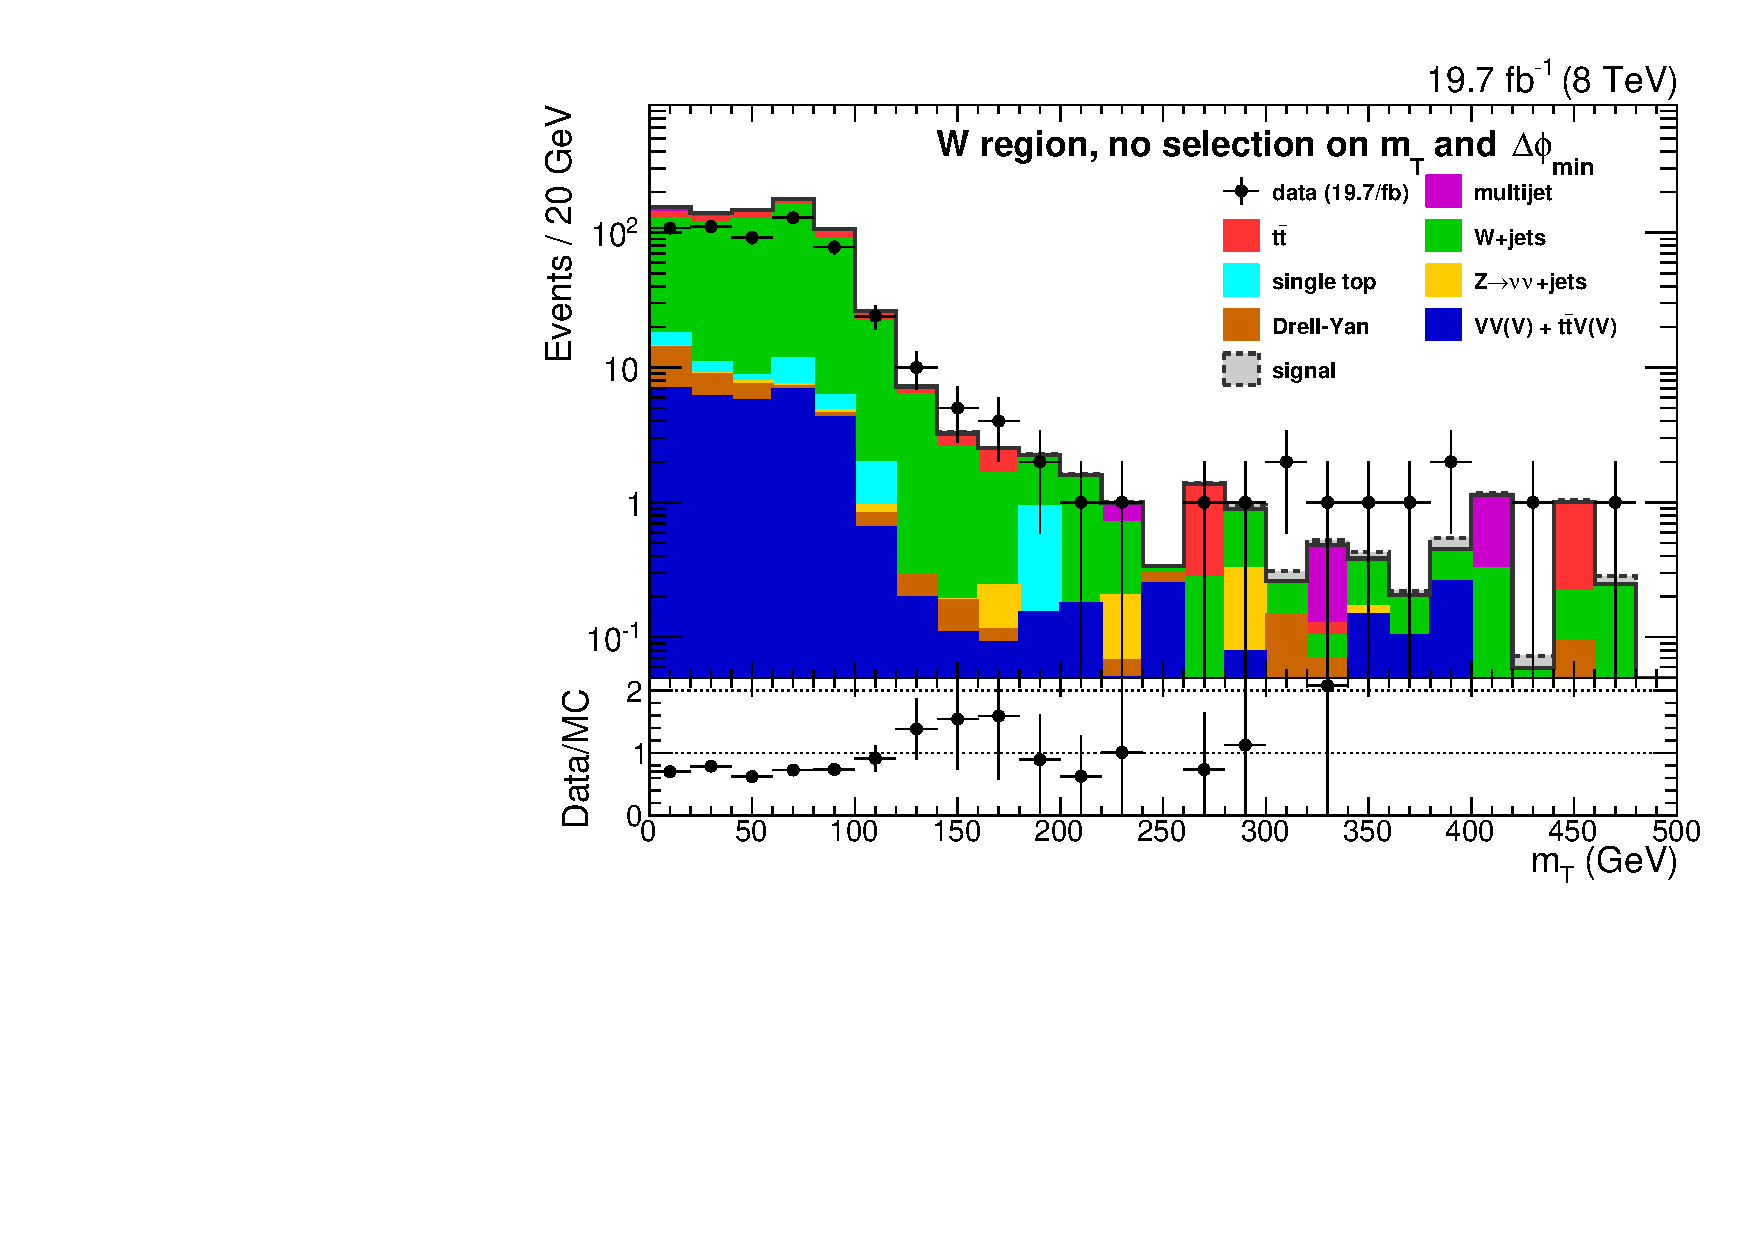
\includegraphics[width=0.49\textwidth]{figures/DataMC/DataMC_mT_0Lbg1Y1Ll_rebin}
% \caption{Comparison between data and simulation for the $m_T$ distribution in the $T$ (left) and
% $W$
% (right) region without applying any selection on $m_T$ and $\Delta\phi_{min}$. An example signal
% point, corresponding to the {\it T1ttcc} mass point with $m_{\tilde{g}} \,{=}\, 1\TeV$,
% $m_{\tilde{t}} \,{=}\, 325\GeV$ and $m_{\tilde{\chi}_1^0} \,{=}\, 300\GeV$, is stacked on top of
% the
% background processes.
% \label{fig:mT}}
% \end{figure}
% 
% \begin{figure}[htbp]
% \centering
%  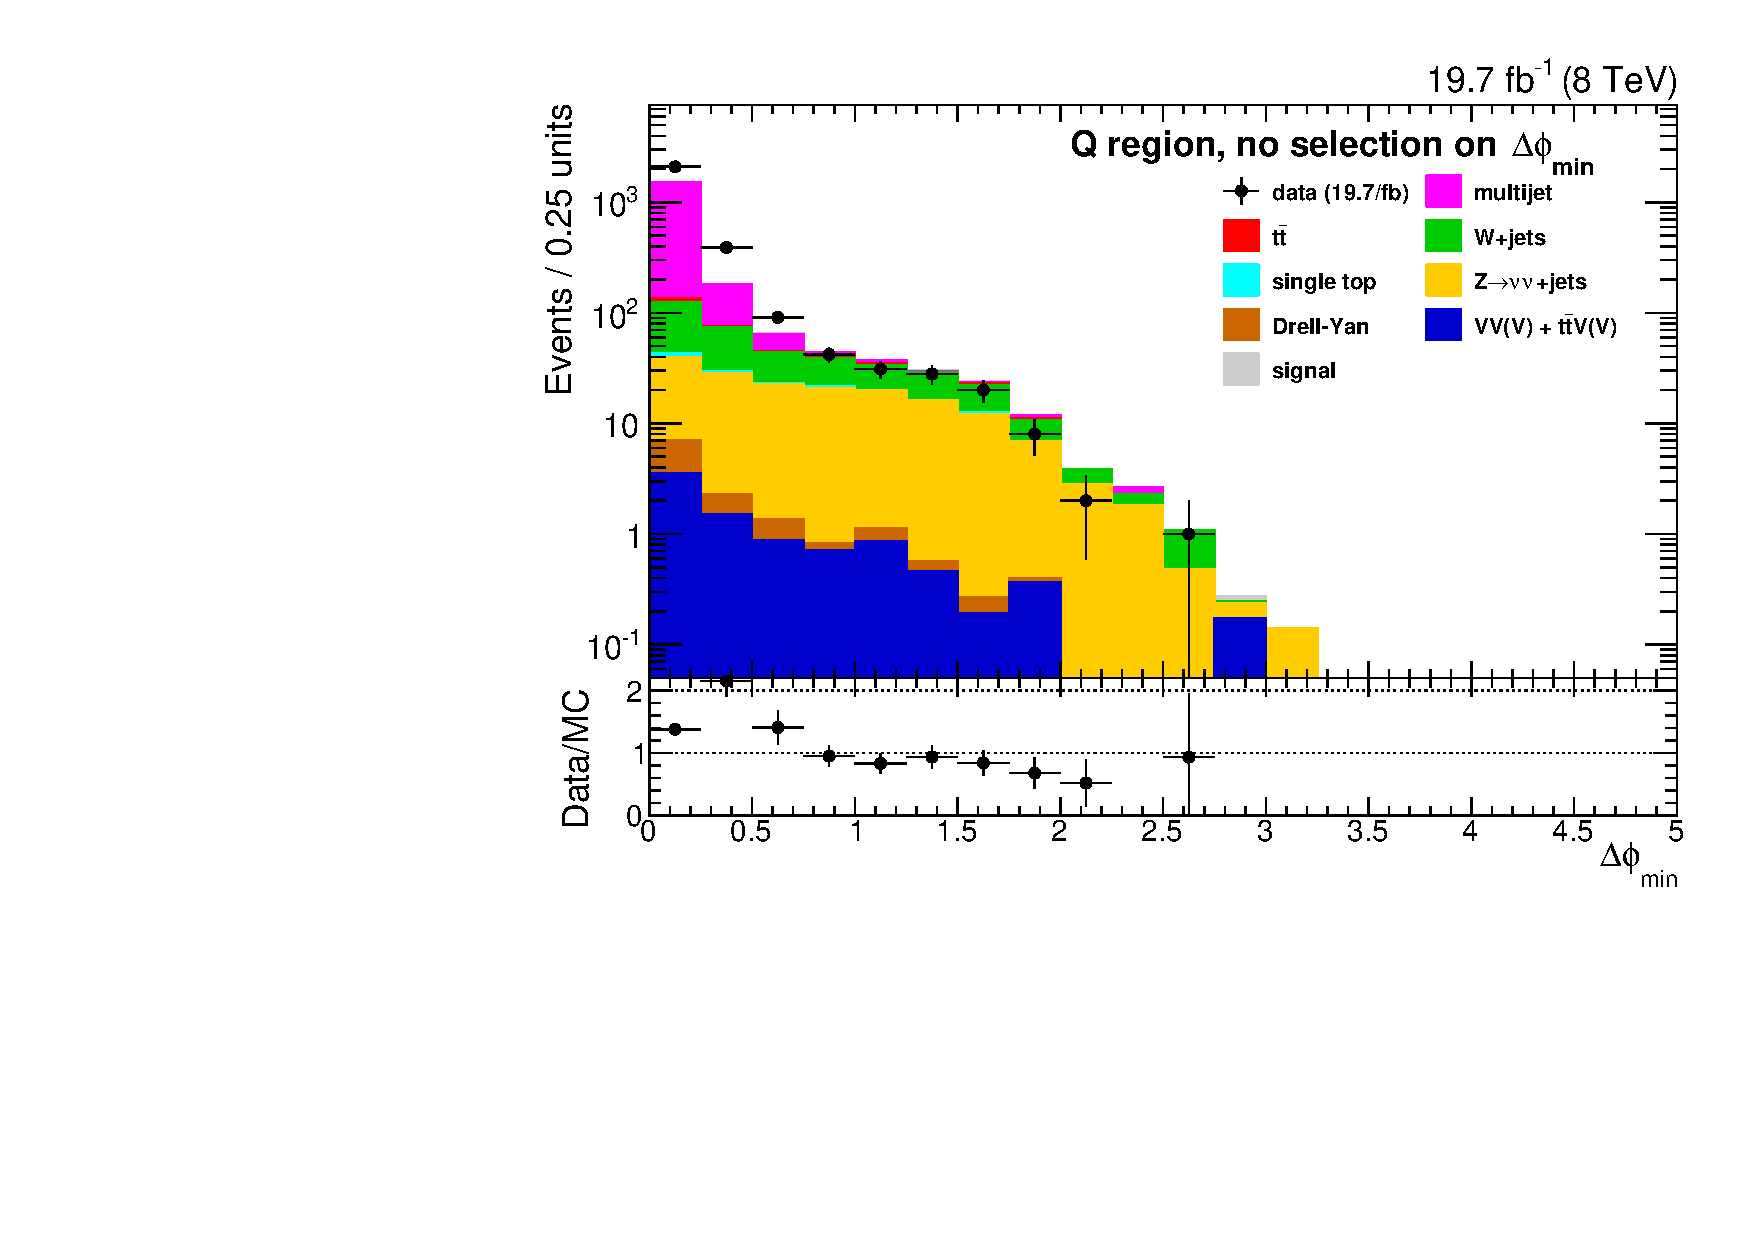
\includegraphics[width=0.49\textwidth]{figures/DataMC/DataMC_minDeltaPhi_0Lbg1uW0Ll_rebin}
% \caption{Comparison between data and simulation for the $\Delta\phi_{min}$ distribution in the $Q$
% region without applying a selection on $\Delta\phi_{min}$. 
% \label{fig:deltaphi}}
% \end{figure}
% 
% 
% In Table~\ref{tab:cutflow}, we show the expected number of events obtained from simulation for the
% different background processes and for an example signal point. The observed events in data for
% the
% selection levels after the trigger requirement are also reported. 
% The background composition in percent after the baseline, $S$, $T$, $W$ and $Q$ region selection
% is
% reported in Table~\ref{tab:BG_comp_percent}.  
% The signal region is $t\bar{t}$ dominated, with additional contributions from $\PW(\rightarrow
% \ell\nu)+$jets and multijet processes. The control regions have a good purity for the background
% process they target: 90\% for multijet, 85\% for $\PW(\rightarrow \ell\nu)+$jets and close to 80\%
% for $t\bar{t}$ and single top processes combined. 





% 
% We also investigated the use of an extension of this variable, called $\Delta\hat{\phi}_{min}$ and
% first used by the RA2b group \cite{RA2b_mdphihat}.
% Originally, we studied these two variables as a way to obtain a cleaner QCD control region, see
% section~\ref{sec:Qregion}. 
% There we found no significant difference between cutting on $\Delta\hat{\phi}_{min}$ or
% $\Delta\phi_{min}$. They can both provide a good separation between QCD and other backgrounds. 
% When testing these variables in the signal region, we found that a cut of $\Delta\phi_{min} > 0.5$
% performed the best in suppressing QCD background. For simplicity we decided to use this variable for
% defining the QCD control region as well. 
%
% The full $\Delta\phi_{min}$ distribution in the signal region is shown in
% figure~\ref{fig:DataMC_SignalRegion_mdphi}.
% In figures~\ref{fig:DataMC_SignalRegion_MR_R2_mdphig0p5} and \ref{fig:DataMC_SignalRegion_mdphig0p5}
% we show a Data/MC comparison for various quantities for the signal region with $\Delta\phi_{min} >
% 0.5$. The \pt distribution of the highest \pt tagged $W$ in the event is shown in
% figure~\ref{fig:Wpt_SignalRegion}.  
% Please note that these plots are for illustration purposes only. 
% We will predict the background using data control regions and only use the simulation for
% translation factors between those control regions and the signal region (see further). We stress in
% particular that the QCD multijet MC is underpredicting what we see in data. 
% 
% \begin{figure}[htbp]
%  \centering
%  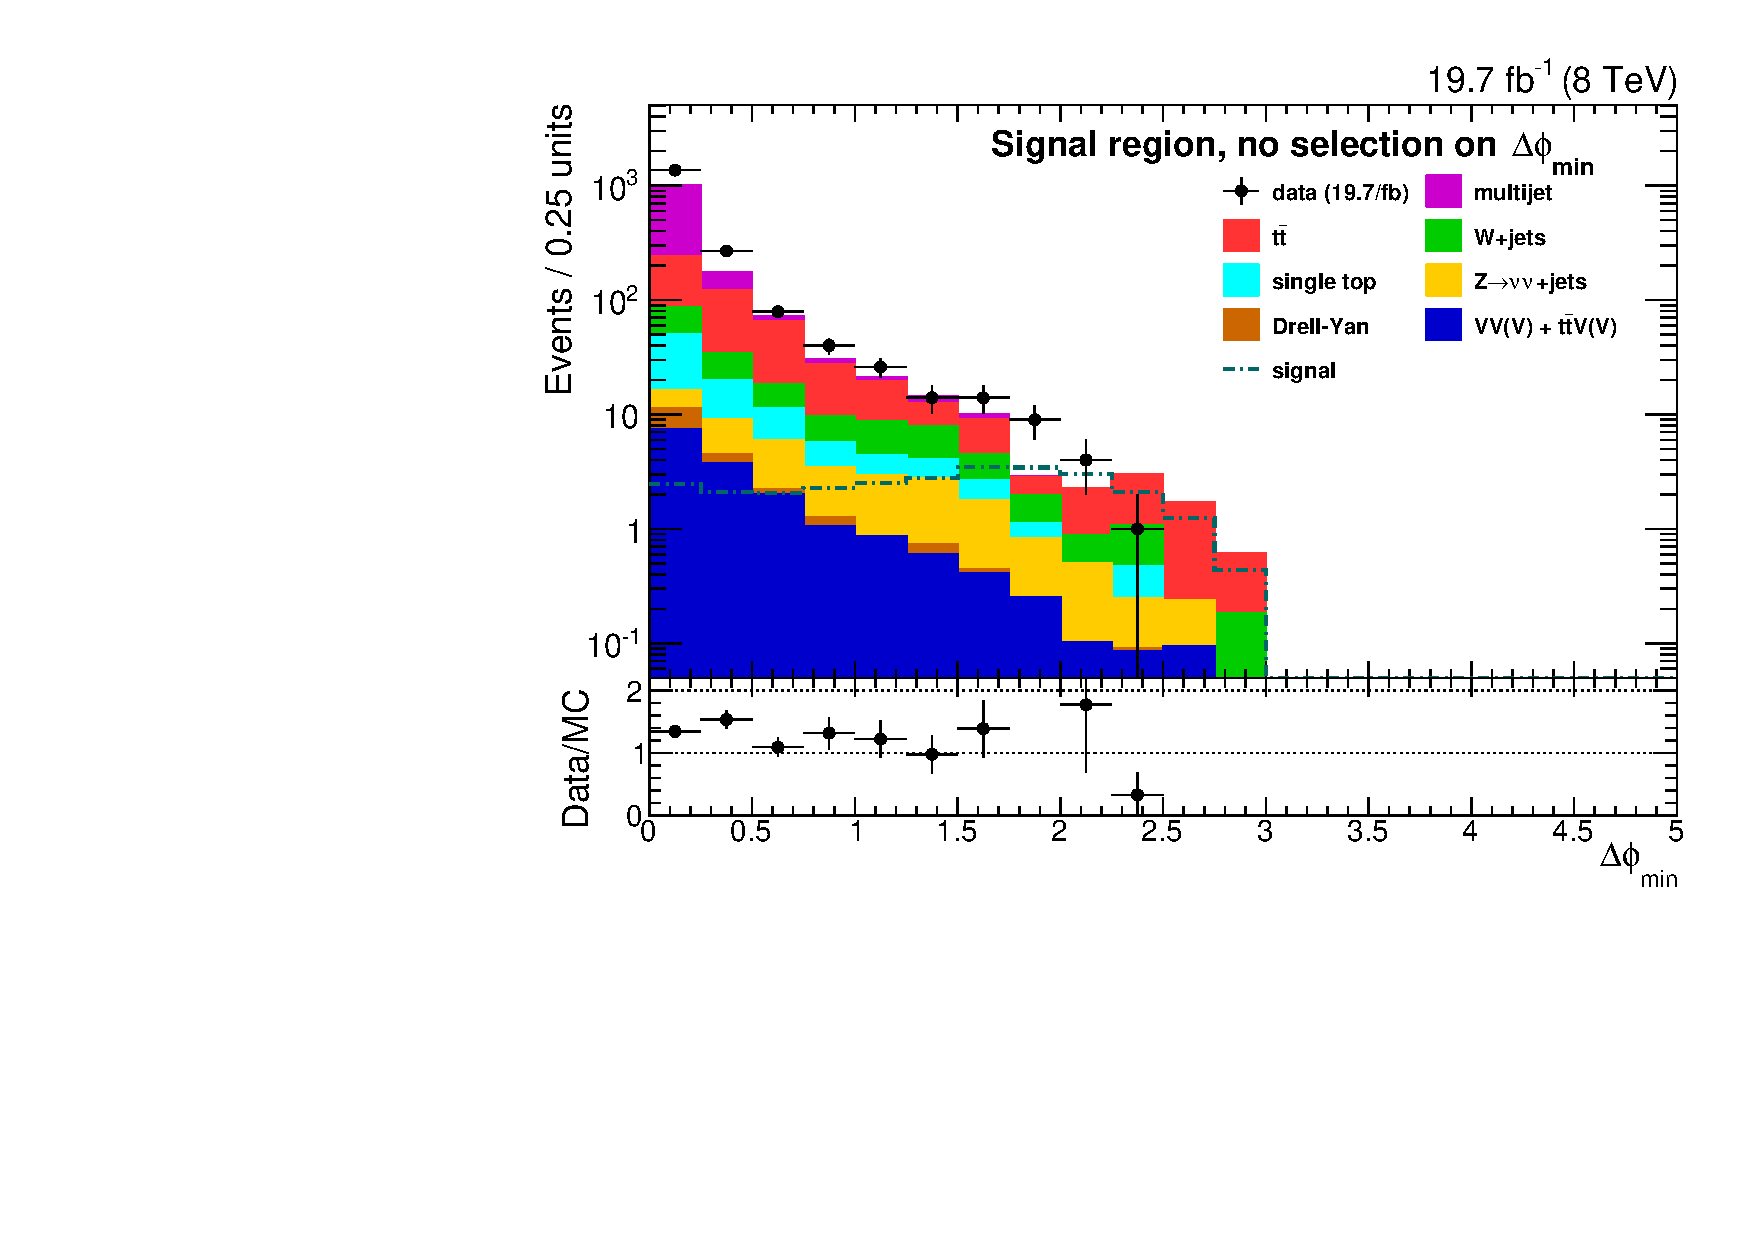
\includegraphics[width=0.49\textwidth]{figures/DataMC/DataMC_minDeltaPhi_g1Mbg1W0Ll_rebin}
% \caption{Data/MC comparison plot for the full $\Delta\phi_{min}$ distribution with all signal region
% requirements applied except $\Delta\phi_{min} > 0.5$.
% \label{fig:DataMC_SignalRegion_mdphi}}
% \end{figure}
% 
% \begin{figure}[htbp]
%  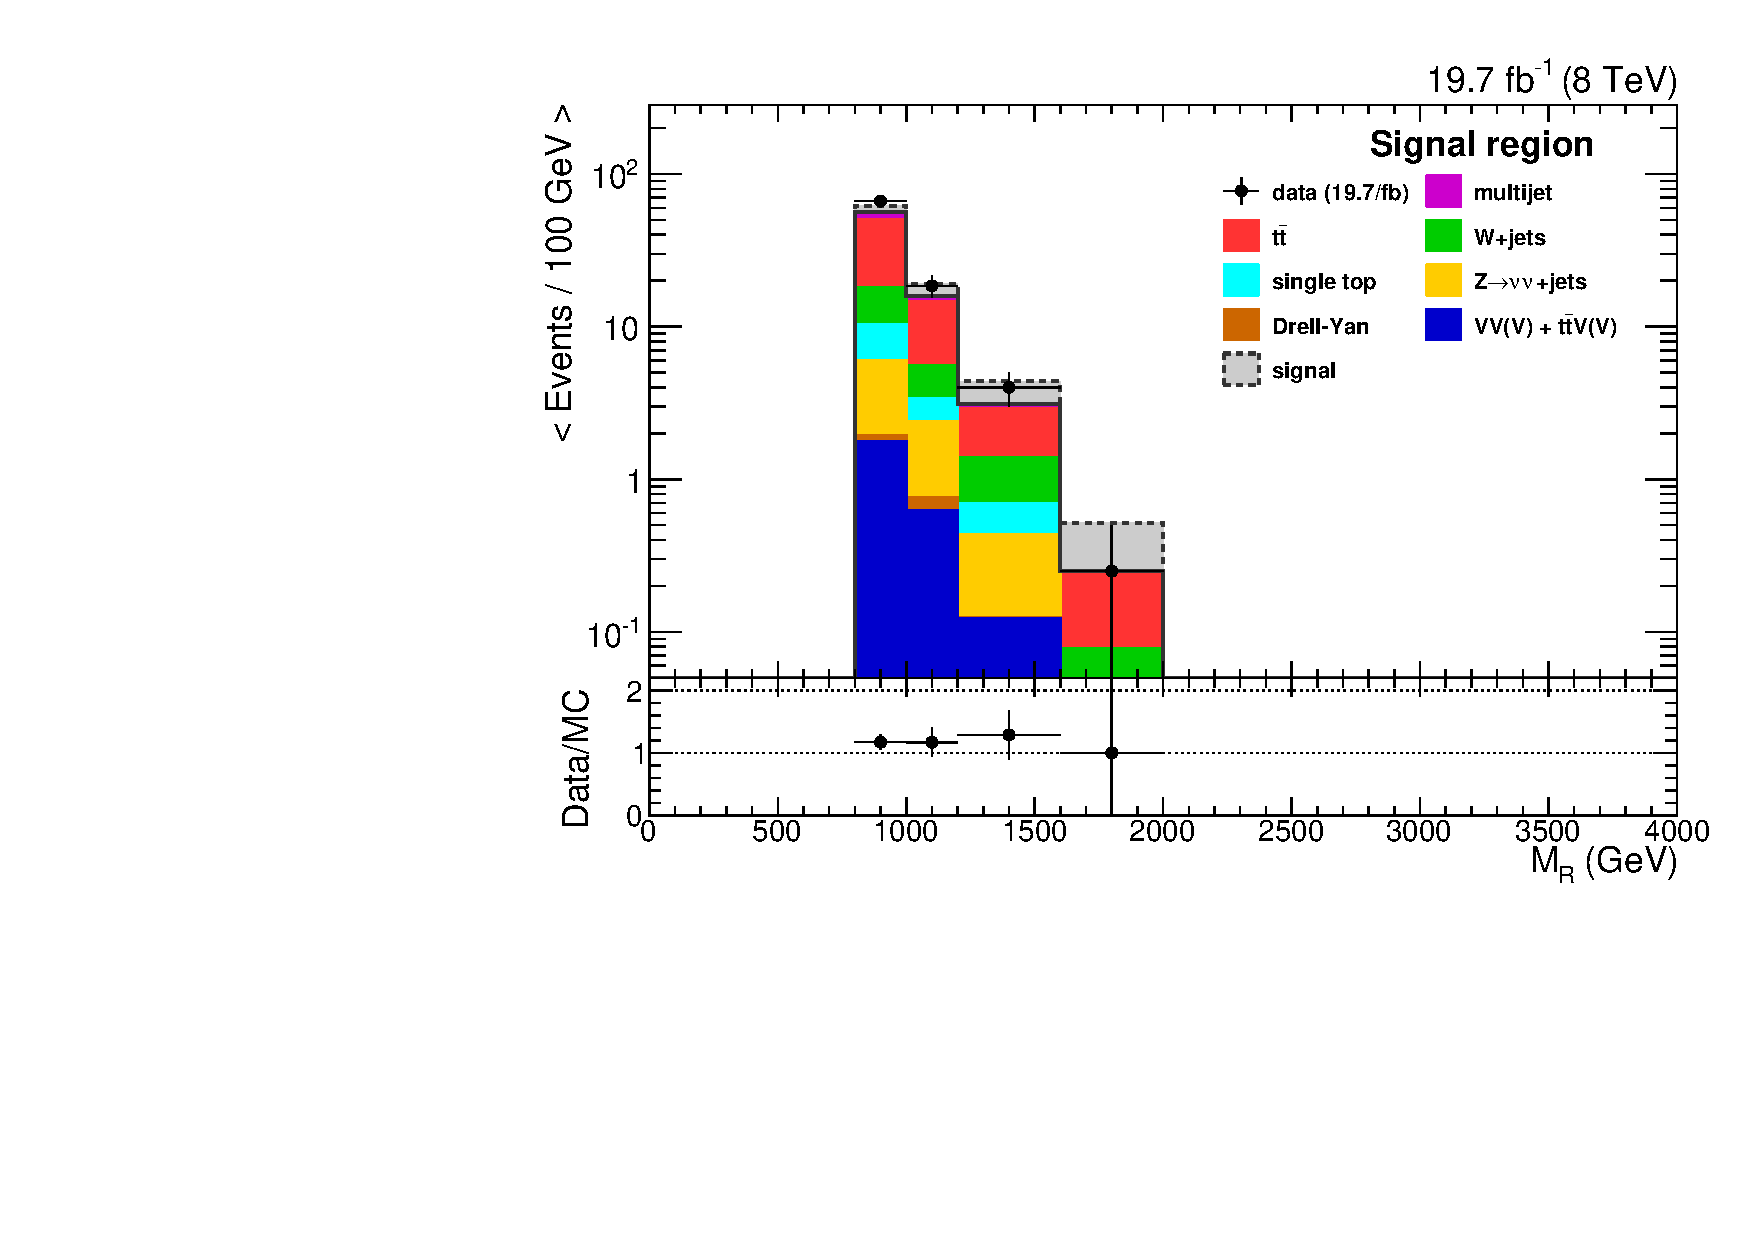
\includegraphics[width=0.49\textwidth]{figures/DataMC/DataMC_MR_g1Mbg1W0Ll_mdPhig0p5_width}
%  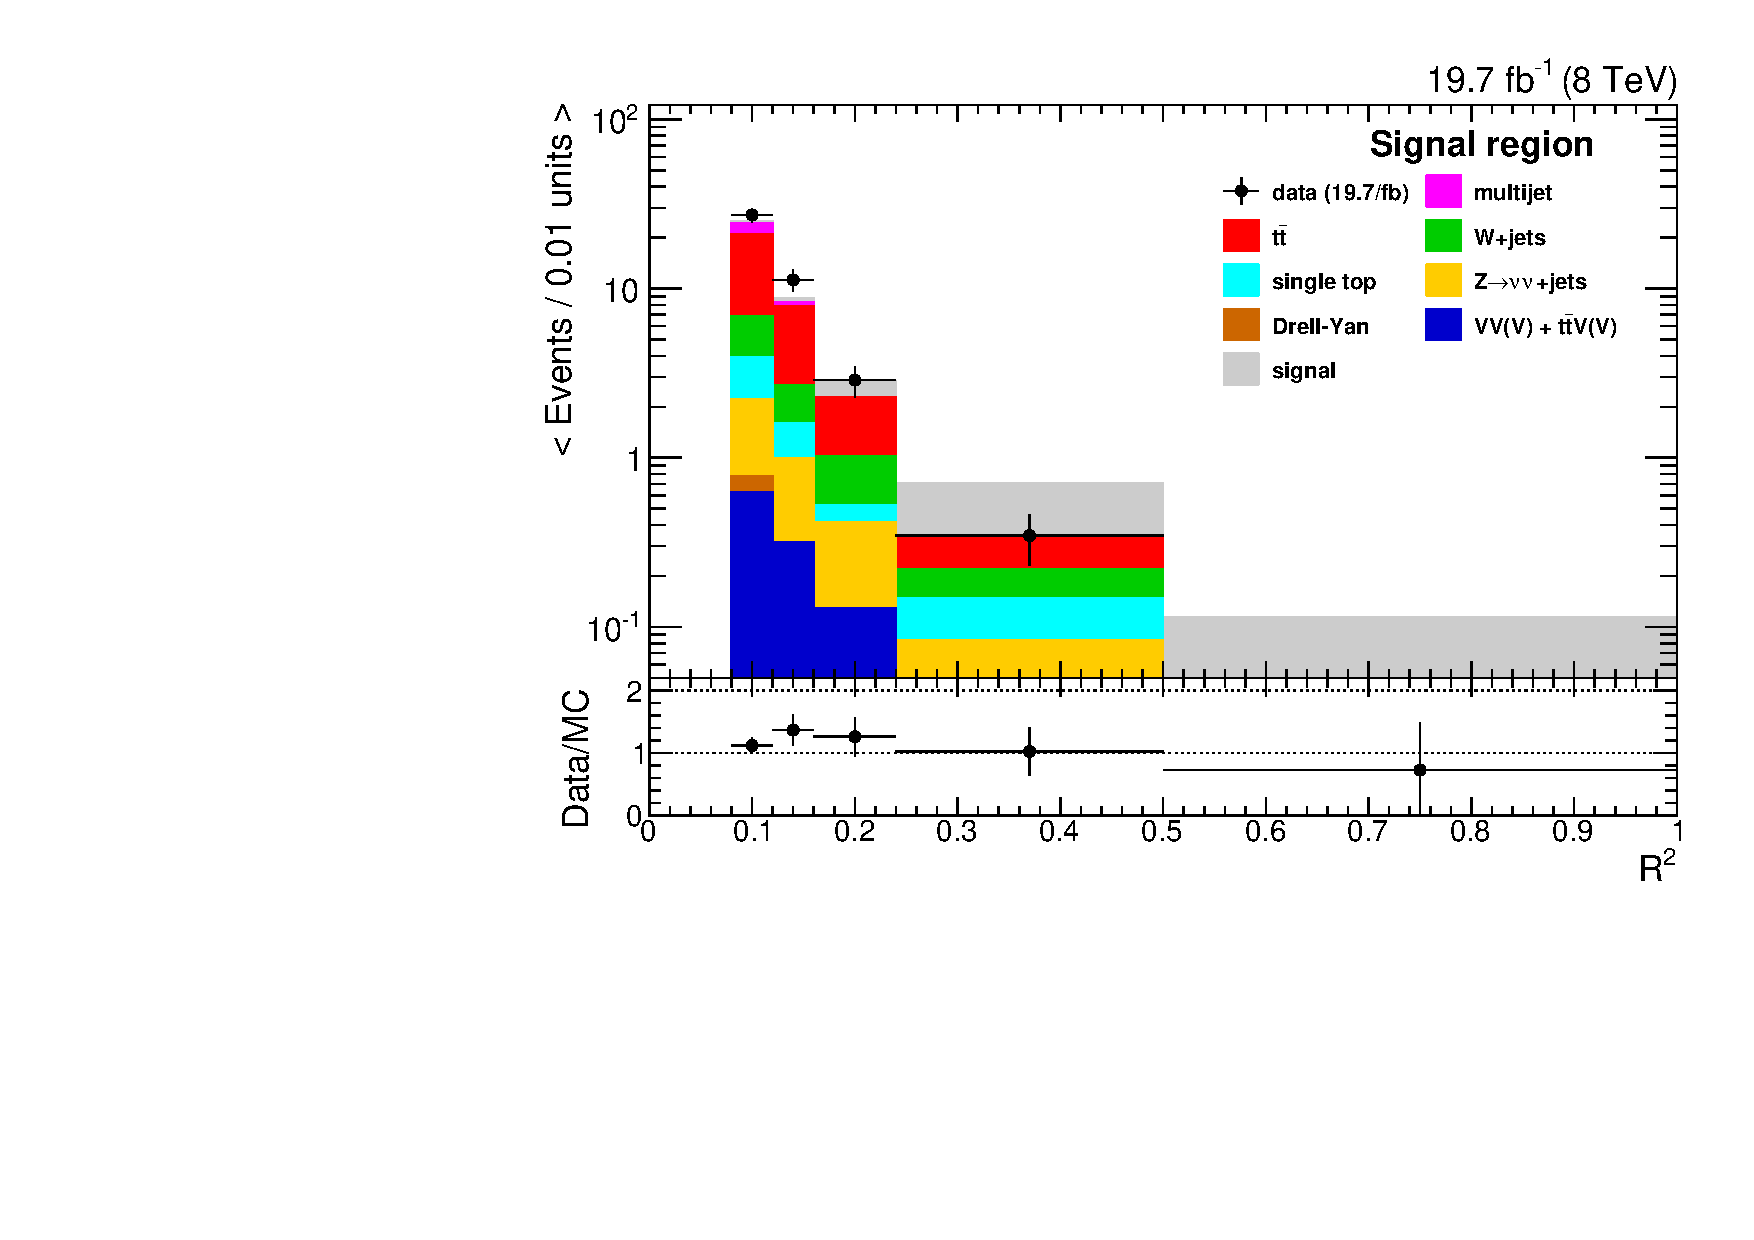
\includegraphics[width=0.49\textwidth]{figures/DataMC/DataMC_R2_g1Mbg1W0Ll_mdPhig0p5_width}
% \caption{For illustration only: Data/MC comparison plot of $M_R$ (left) and $R^2$ (right) in the
% signal region requiring $\Delta\phi_{min} > 0.5$.
% \label{fig:DataMC_SignalRegion_MR_R2_mdphig0p5}}
% \end{figure}
% 
% 
% \begin{figure}[p]
%  \includegraphics[width=0.49\textwidth]{figures/DataMC/DataMC_njets_g1Mbg1W0Ll_mdPhig0p5}
%  \includegraphics[width=0.49\textwidth]{figures/DataMC/DataMC_nbjets_g1Mbg1W0Ll_mdPhig0p5}
% 
%  \includegraphics[width=0.49\textwidth]{figures/DataMC/DataMC_met_g1Mbg1W0Ll_mdPhig0p5}
%  \includegraphics[width=0.49\textwidth]{figures/DataMC/DataMC_jet1pt_g1Mbg1W0Ll_mdPhig0p5}
% 
%  \includegraphics[width=0.49\textwidth]{figures/DataMC/DataMC_jet2pt_g1Mbg1W0Ll_mdPhig0p5}
%  \includegraphics[width=0.49\textwidth]{figures/DataMC/DataMC_jet3pt_g1Mbg1W0Ll_mdPhig0p5}
% \caption{For illustration only: Data/MC comparison plot of various event quantities in the signal
% region requiring $\Delta\phi_{min} > 0.5$: 
% [top] jet multiplicity (left) and b-tagged jet multiplicity (right);
% [middle] missing transverse energy (left) and \pt of the highest \pt jet (right);
% [bottom] \pt of the second (left) and third (right) highest \pt jet. 
% \label{fig:DataMC_SignalRegion_mdphig0p5}}
% \end{figure}
% 
% \begin{figure}[htbp]
%  \includegraphics[width=0.49\textwidth]{figures/DataMC/DataMC_Wpt_g1Mbg1W0Ll_mdPhig0p5}
%  \includegraphics[width=0.49\textwidth]{figures/Shapes/comparison_Wpt}
% \caption{For illustration only: [left] Data/MC comparison plot of $\pt(W)$ in the signal region
% requiring $\Delta\phi_{min} > 0.5$.
% [right] Comparison of the $\pt(W)$ distribution for signal and total background. Both distributions
% are normalized to unit area.
% \label{fig:Wpt_SignalRegion}}
% \end{figure}
% 
% To get a sense of the signal sensitivity we can expect, we show the signal efficiencies, expected
% number of events and significances $\frac{S}{\sqrt{B}}$ for the T1ttcc simplified model in
% figure~\ref{fig:eff_T1ttcc}, for the T1t1t model in figure~\ref{fig:eff_T1t1t} and for the T2tt
% model in figure~\ref{fig:eff_T2tt}. 
% Efficiencies of up to 7\% in the most boosted regimes of these scans are reached. 
% For the T1ttcc model a drop in efficiency is observed for the strip with lowest neutralino mass
% ($m_{\chi_1^0} = 1\GeV$). 
% For strips with higher LSP masses, the LSP will end up with higher momentum than the charm. For the
% lowest LSP mass however, the LSP and the charm have about equal mass, so after the boost they will
% receive about equal amounts of momentum. This results in a lower \ETm spectrum, and in the end a
% lower efficiency. 
% This is explained in more detail in Appendix~\ref{app:eff_drop}. 
% 
% \begin{figure}[htbp]
%  \centering
%  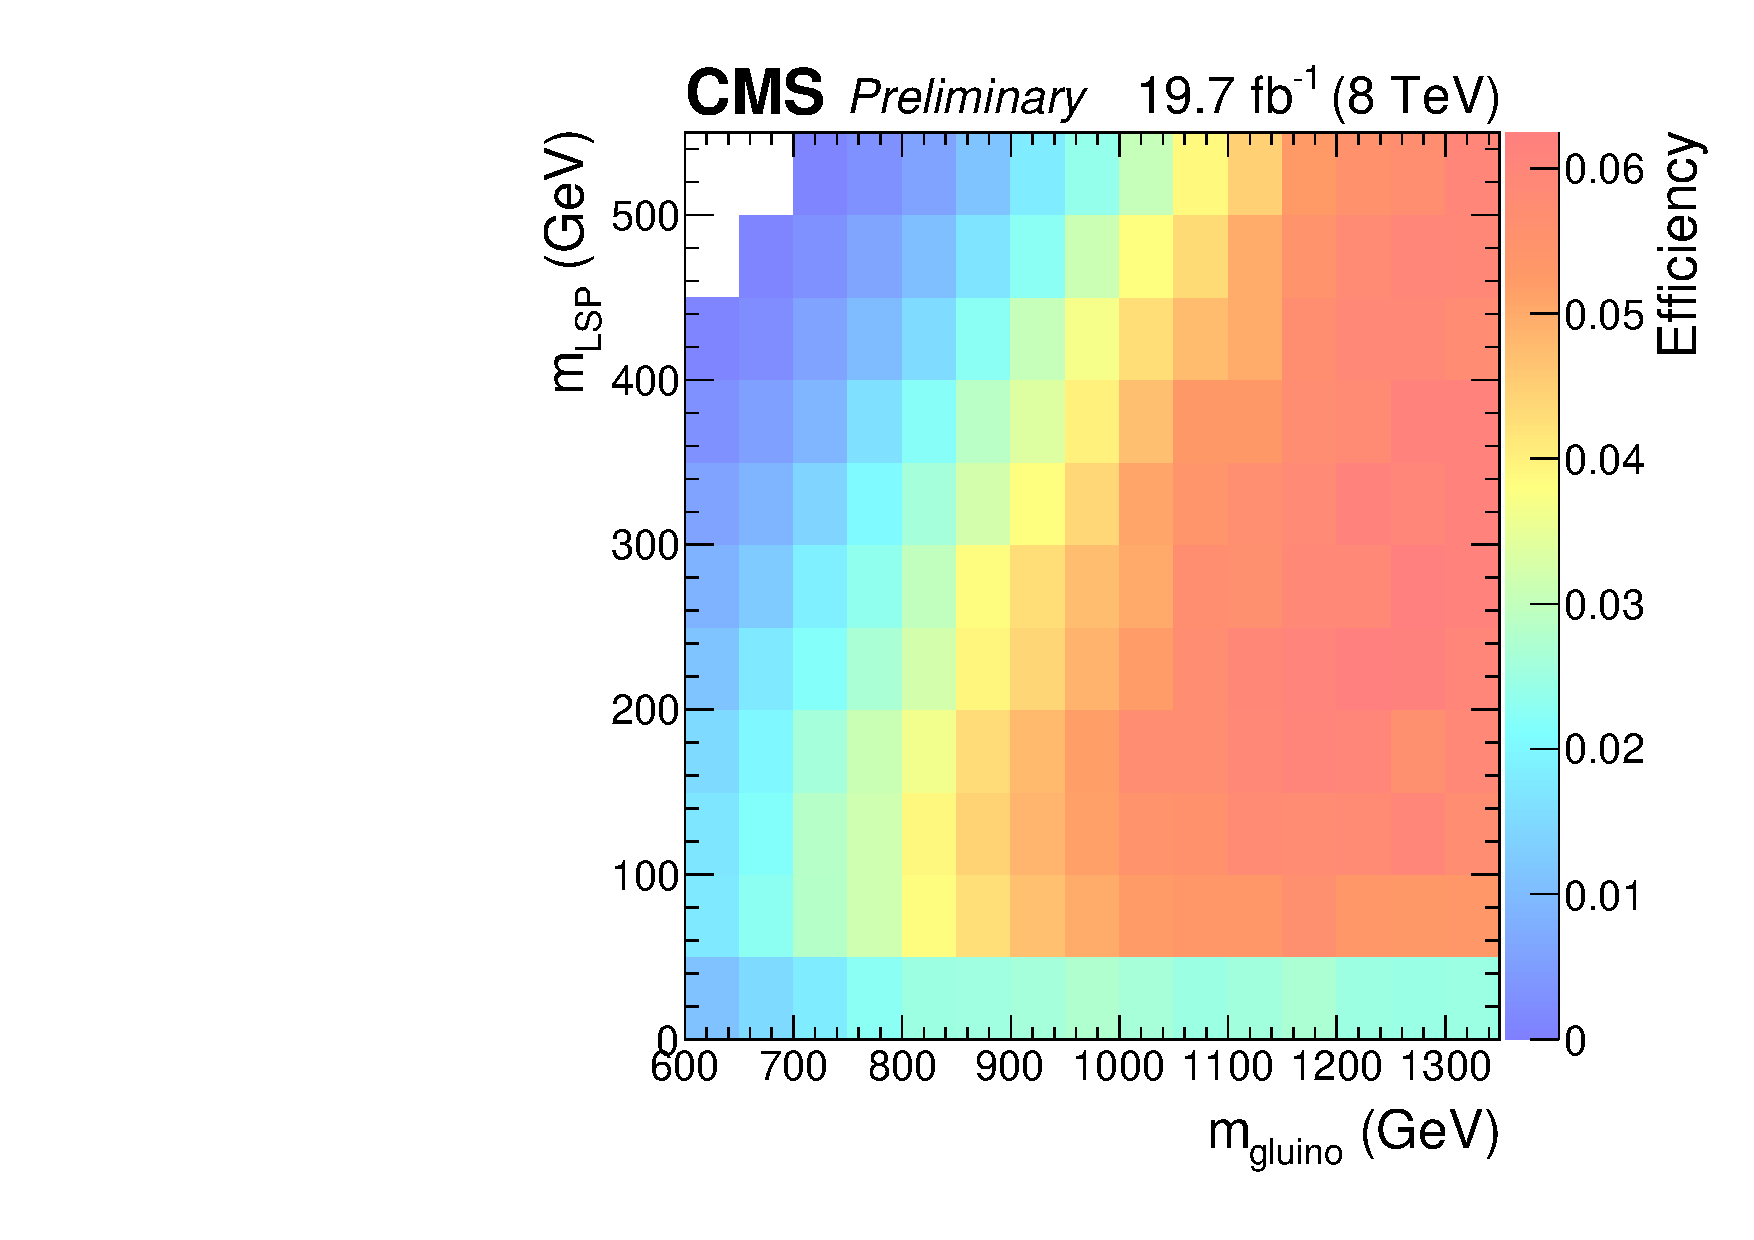
\includegraphics[width=0.3\textwidth]{figures/T1ttcc/efficiency_T1ttcc_DM-10_g1Mbg1W0Ll_mdPhig0p5}
% ~
%  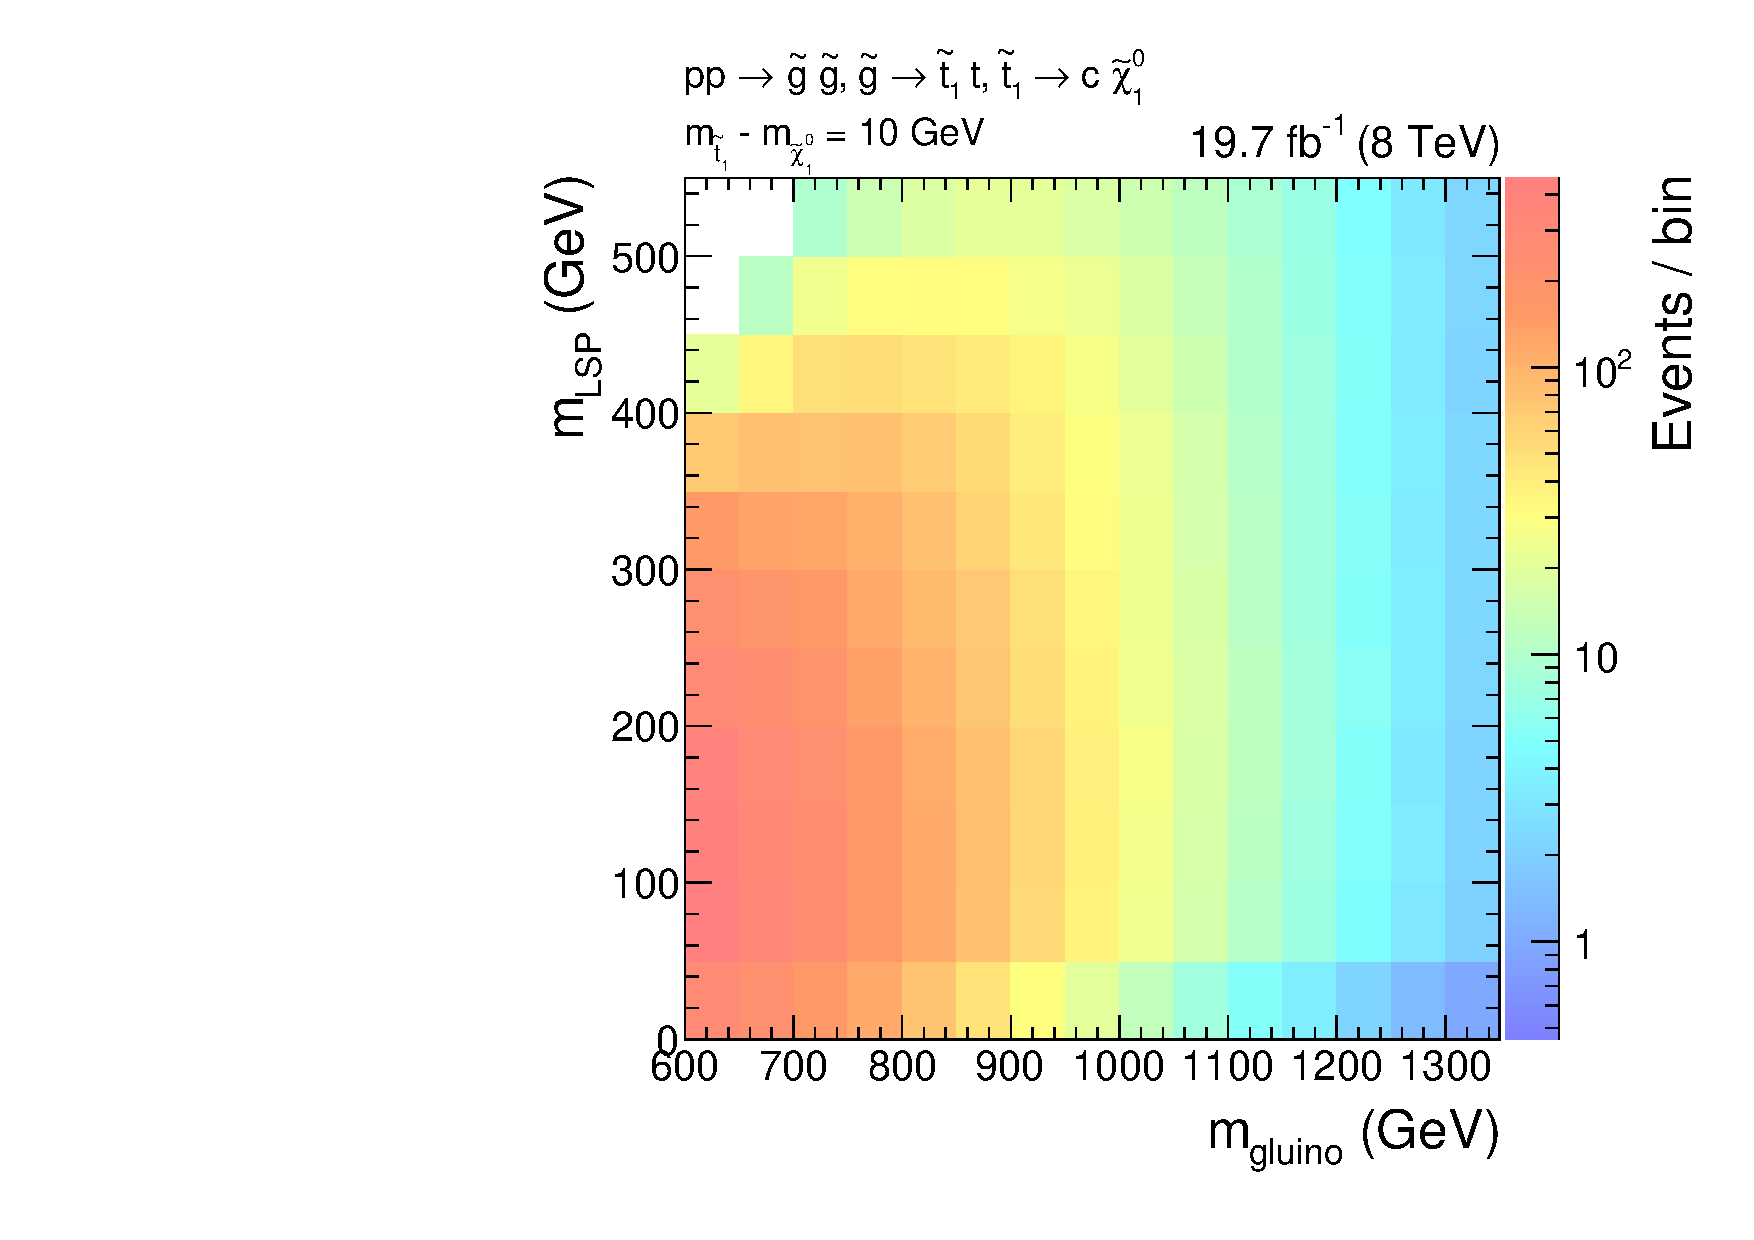
\includegraphics[width=0.3\textwidth]{figures/T1ttcc/events_T1ttcc_DM-10_g1Mbg1W0Ll_mdPhig0p5} ~
%  \includegraphics[width=0.3\textwidth]{figures/T1ttcc/significance_T1ttcc_DM-10_g1Mbg1W0Ll_mdPhig0p5
% }
% 
%  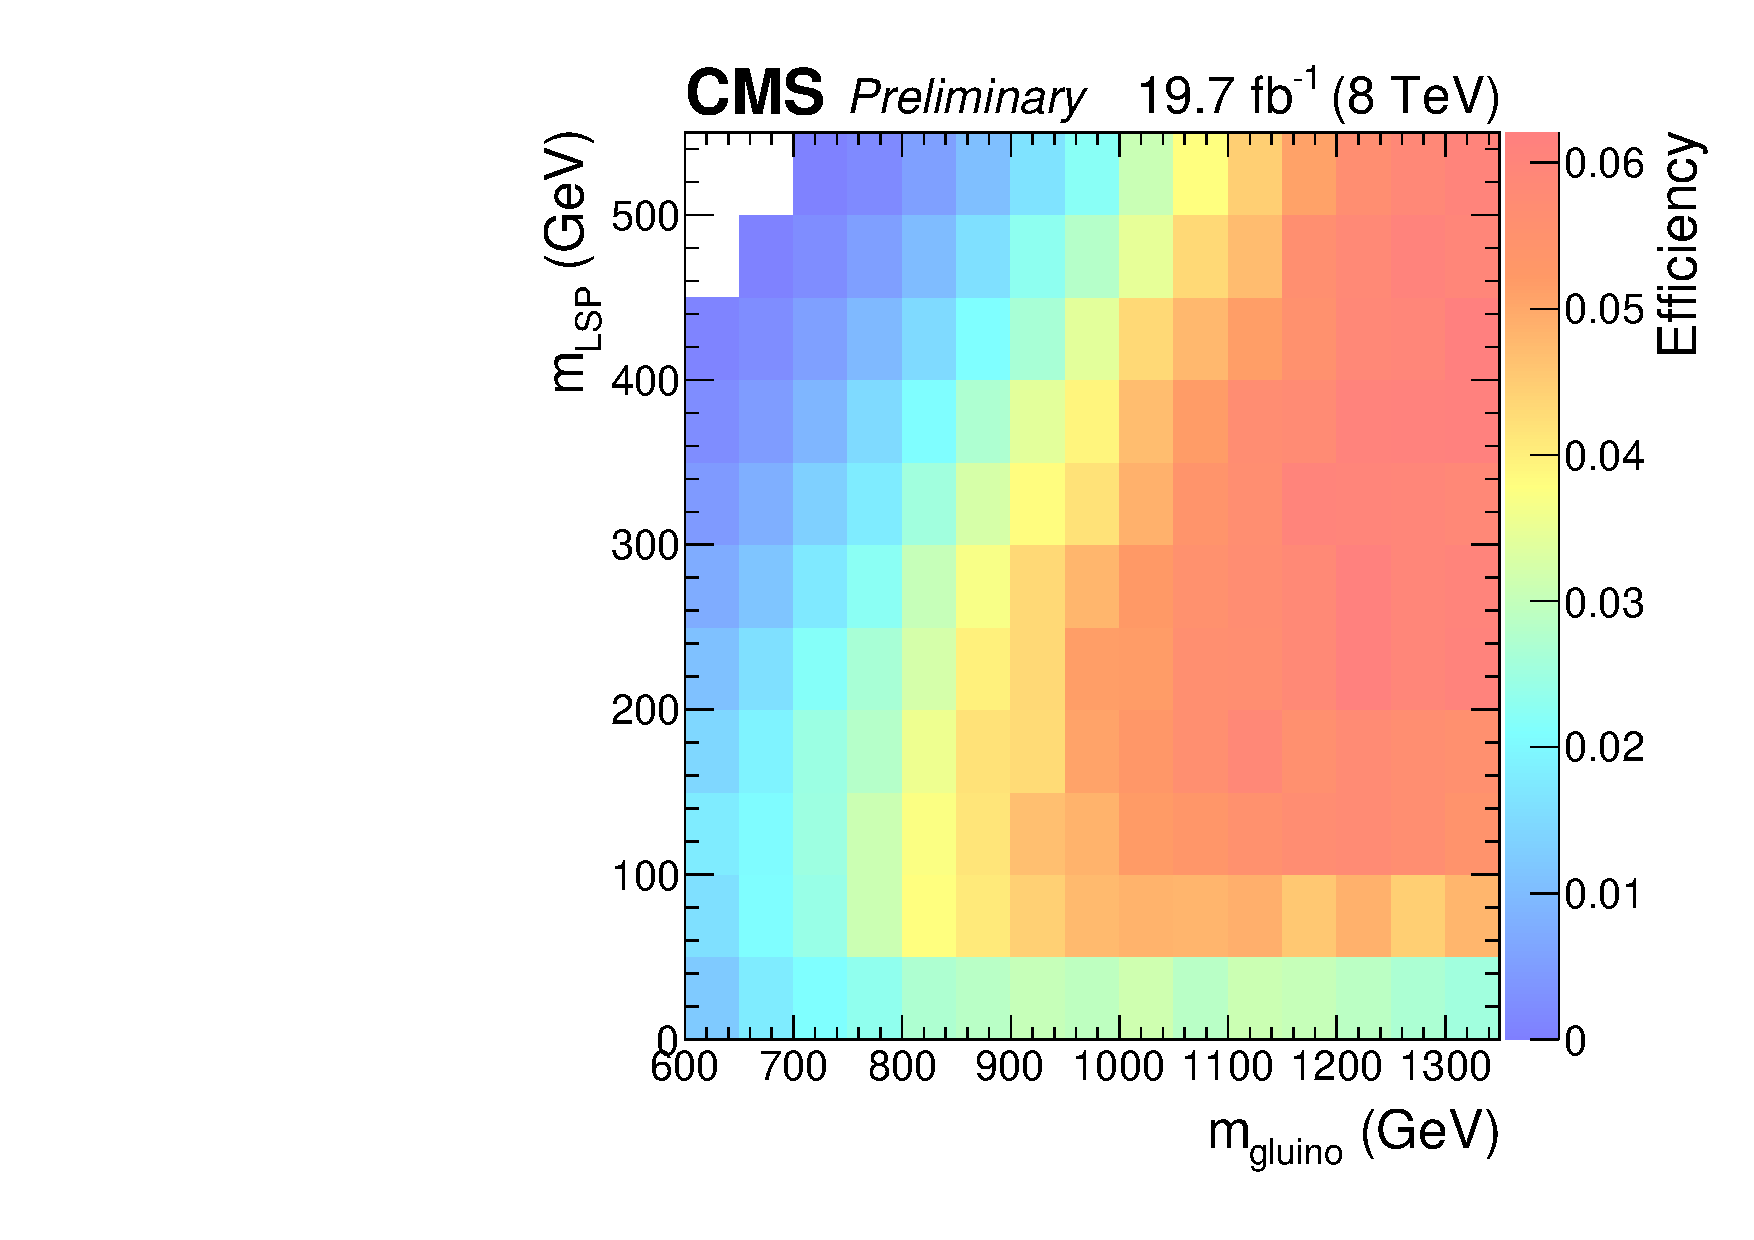
\includegraphics[width=0.3\textwidth]{figures/T1ttcc/efficiency_T1ttcc_DM-25_g1Mbg1W0Ll_mdPhig0p5}
% ~
%  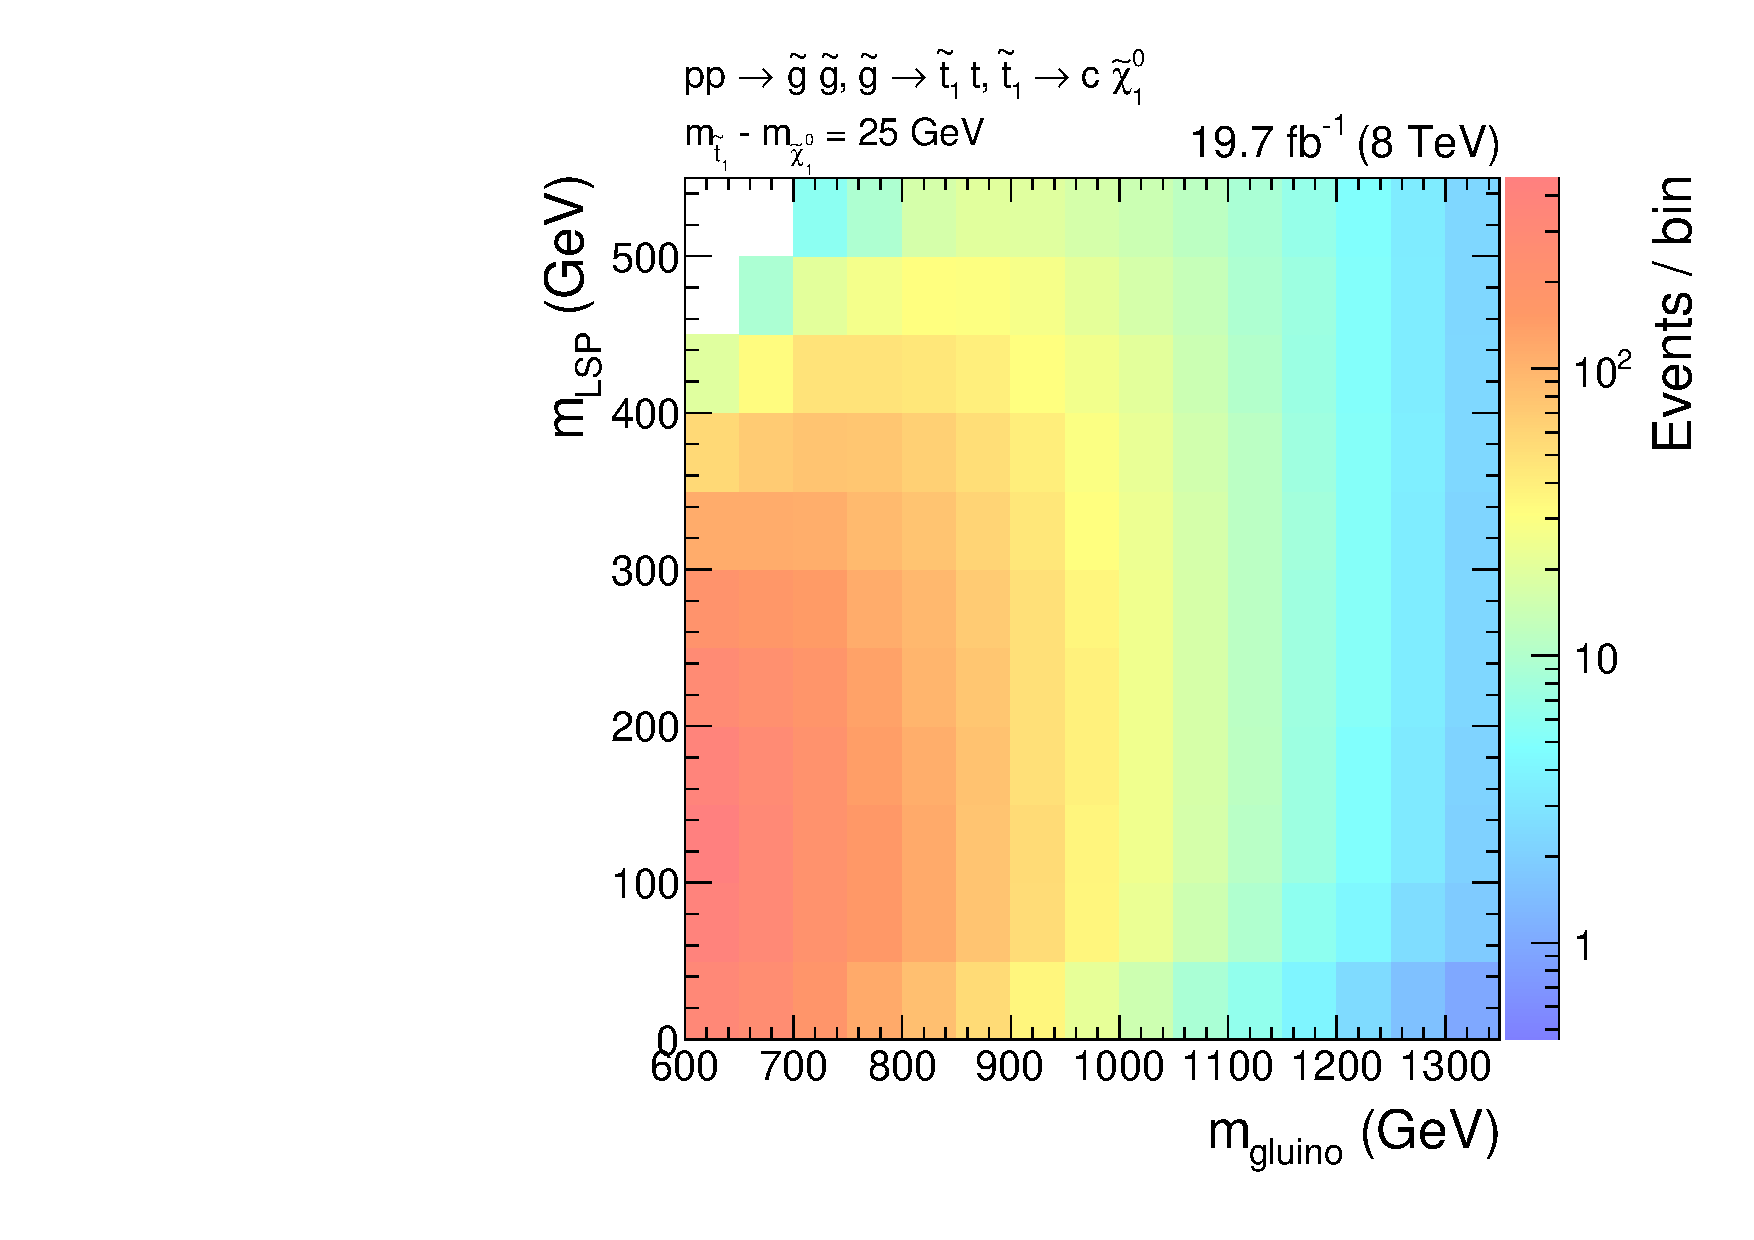
\includegraphics[width=0.3\textwidth]{figures/T1ttcc/events_T1ttcc_DM-25_g1Mbg1W0Ll_mdPhig0p5} ~
%  \includegraphics[width=0.3\textwidth]{figures/T1ttcc/significance_T1ttcc_DM-25_g1Mbg1W0Ll_mdPhig0p5
% }
% 
%  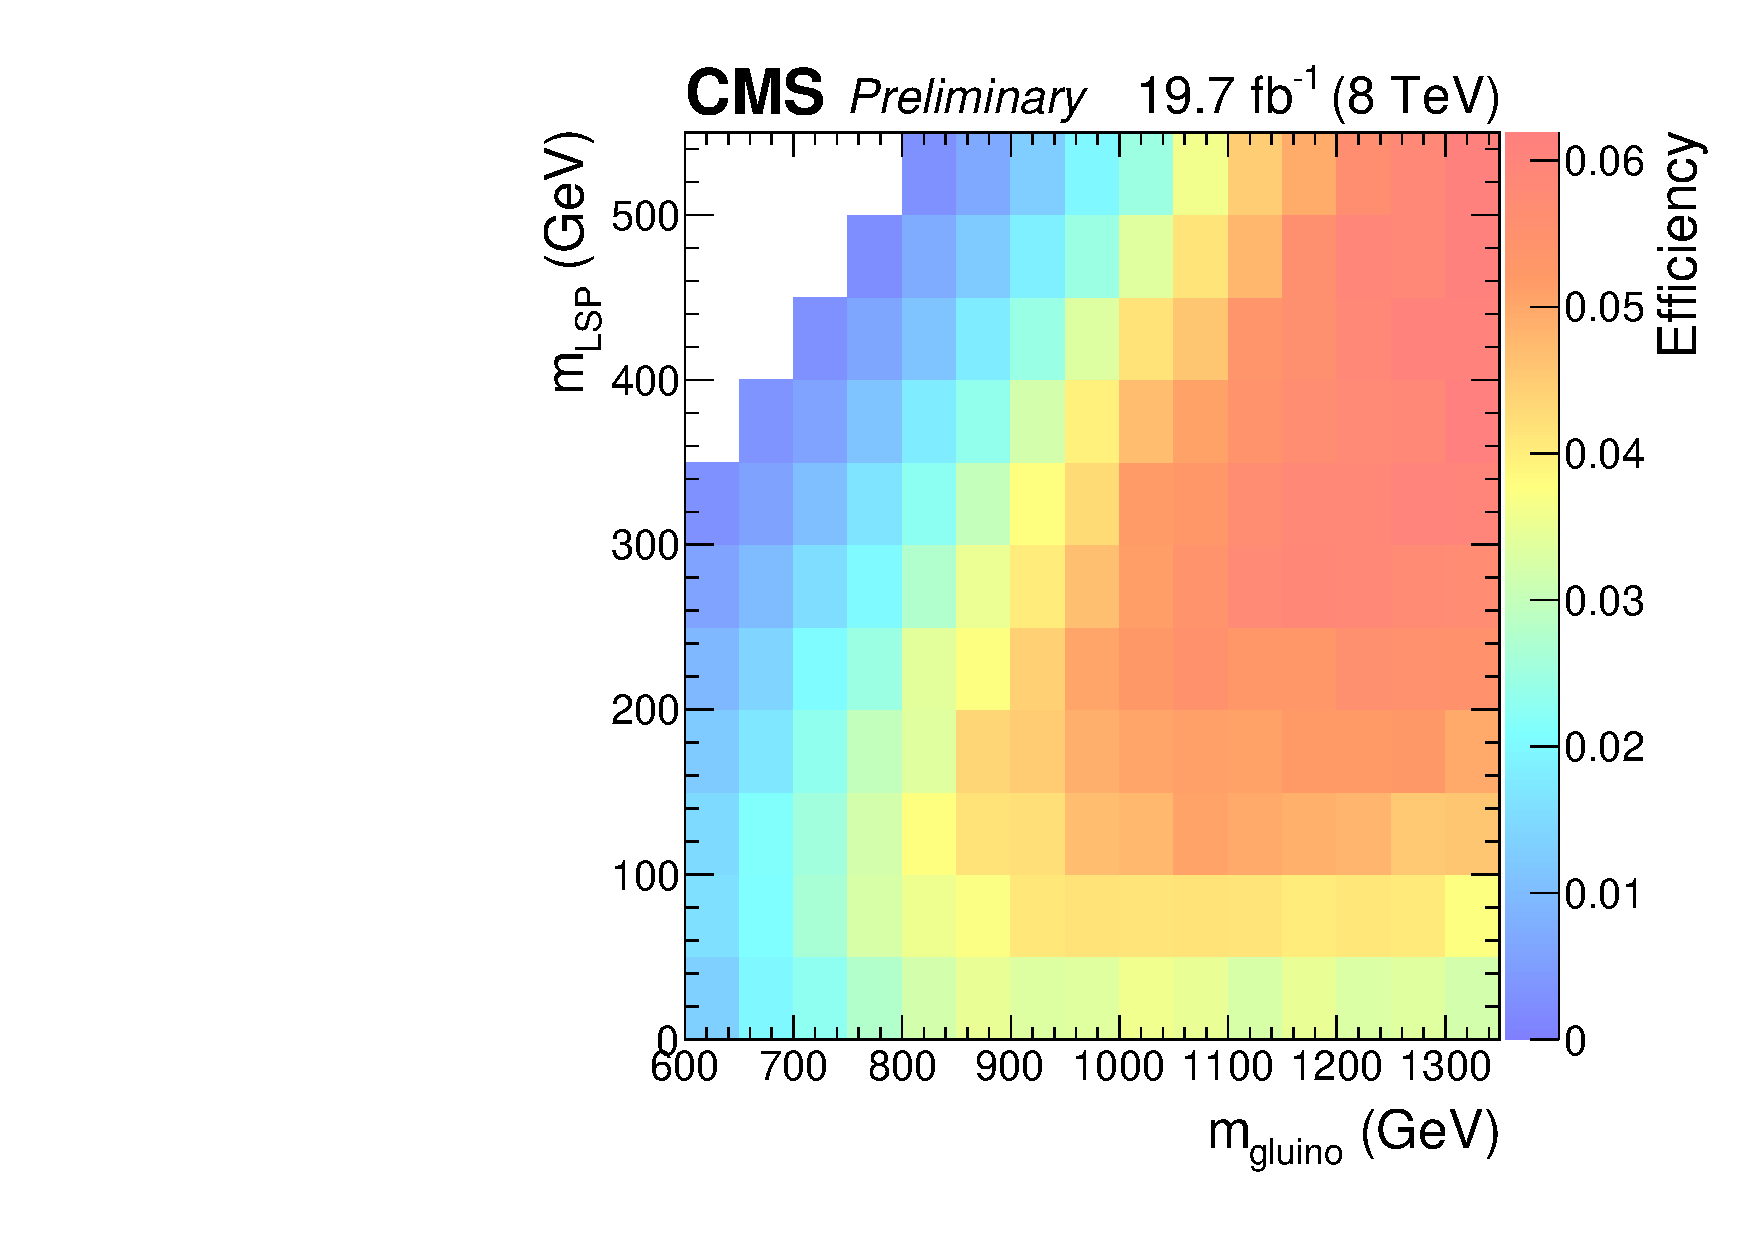
\includegraphics[width=0.3\textwidth]{figures/T1ttcc/efficiency_T1ttcc_DM-80_g1Mbg1W0Ll_mdPhig0p5}
% ~
%  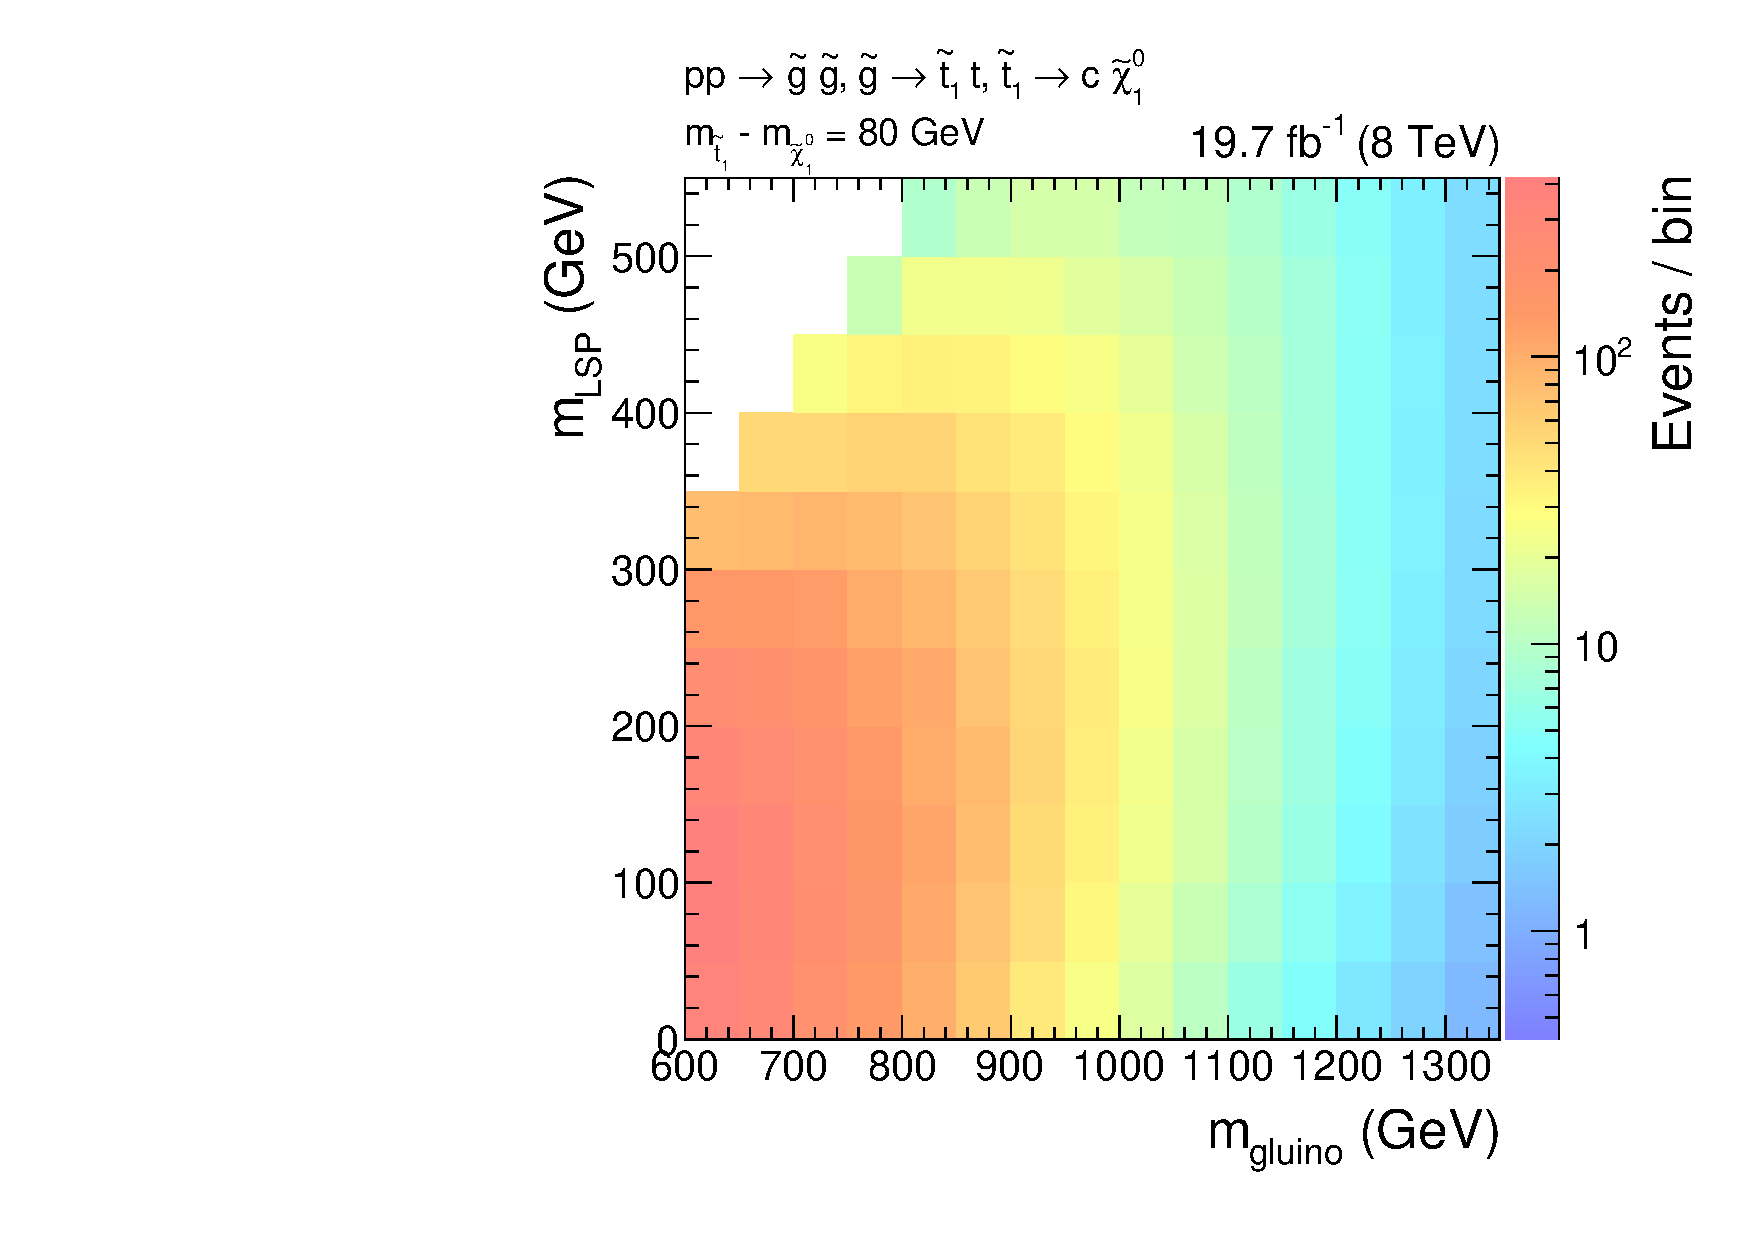
\includegraphics[width=0.3\textwidth]{figures/T1ttcc/events_T1ttcc_DM-80_g1Mbg1W0Ll_mdPhig0p5} ~
%  \includegraphics[width=0.3\textwidth]{figures/T1ttcc/significance_T1ttcc_DM-80_g1Mbg1W0Ll_mdPhig0p5
% }
%  \caption{Signal region efficiency, number of events in $19.712\textrm{fb}^{-1}$ and significance
% $\frac{S}{\sqrt{B}}$ for the T1ttcc simplified model. Three mass splittings between stop and LSP are
% considered: 10, 25 and 80 \GeV, shown in the top, middle and bottom row, respectively.
%  \label{fig:eff_T1ttcc}}
% \end{figure}
% 
% \begin{figure}[htbp]
%  \centering
%   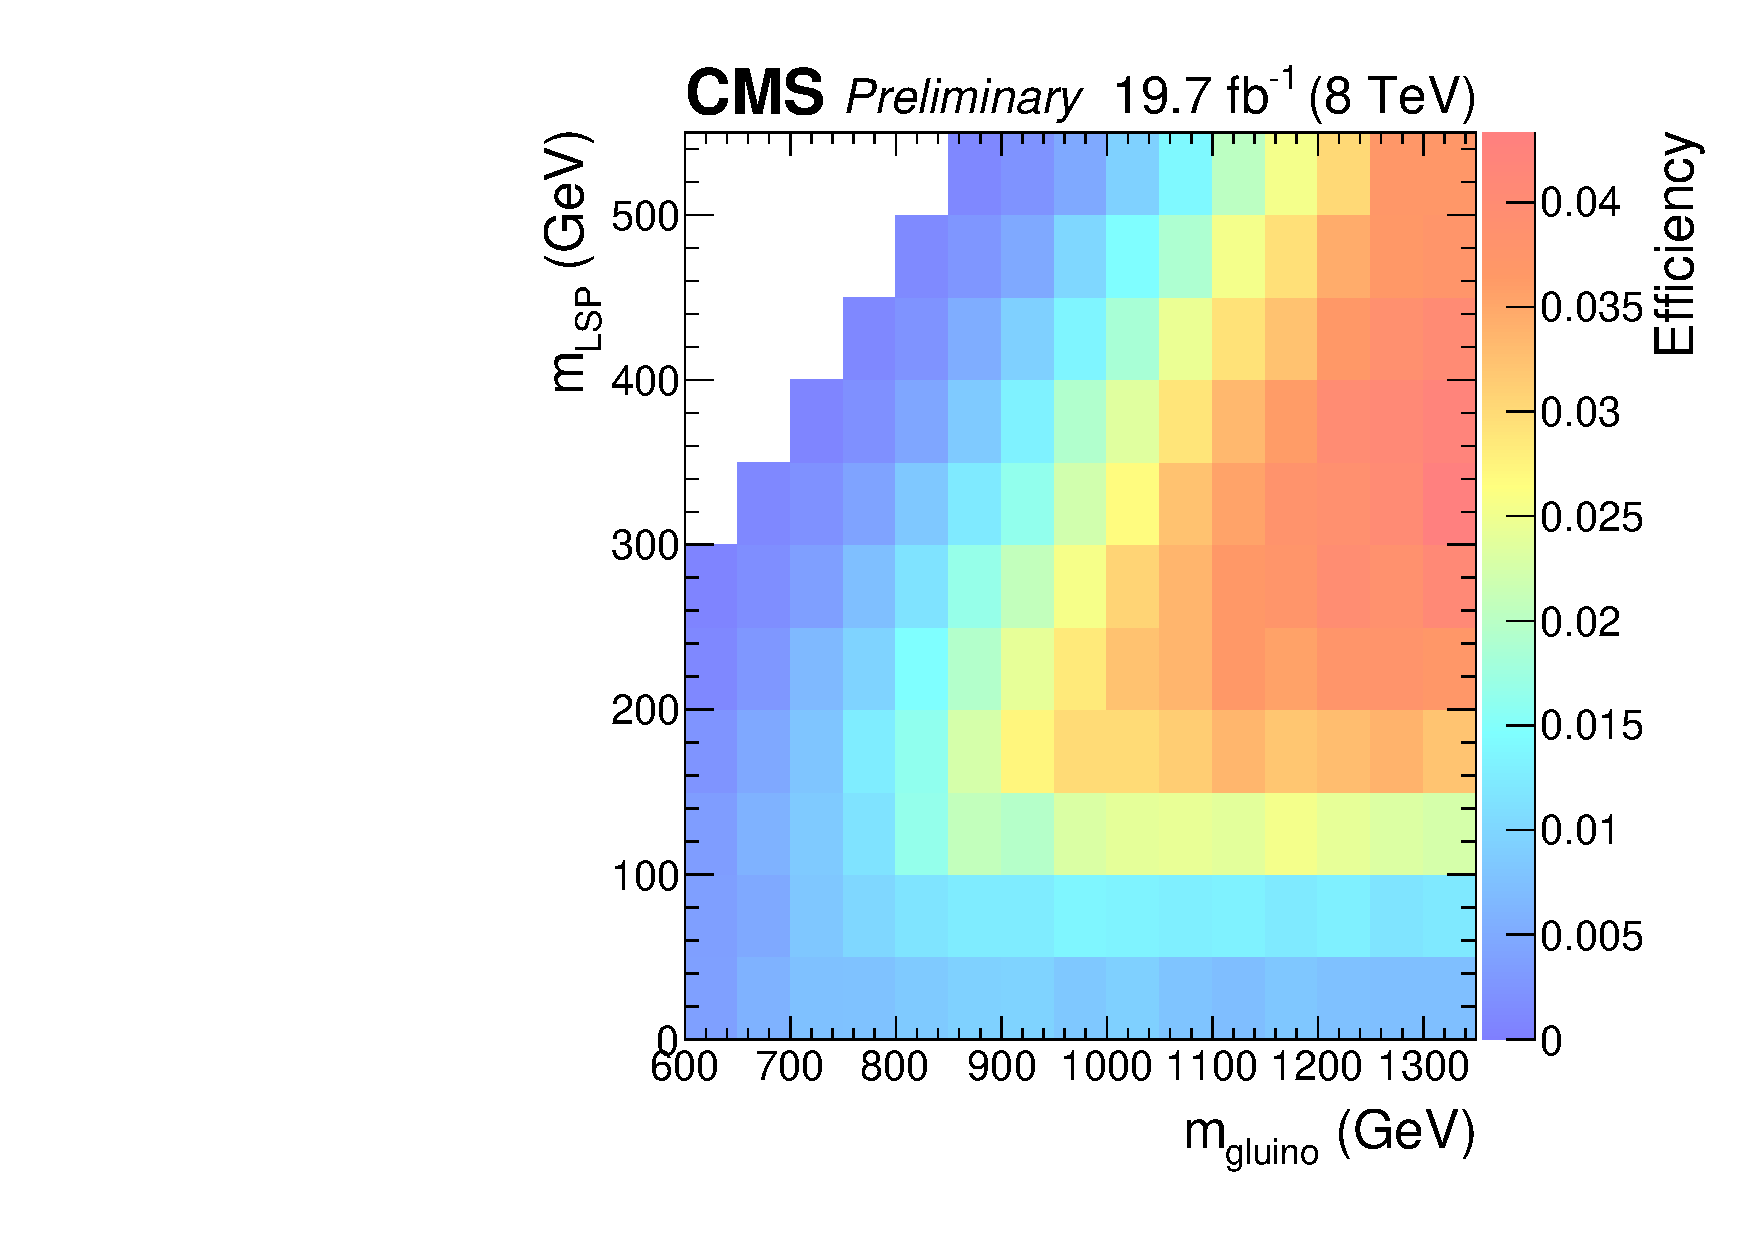
\includegraphics[width=0.3\textwidth]{figures/T1t1t/efficiency_T1t1t_g1Mbg1W0Ll_mdPhig0p5} ~
%  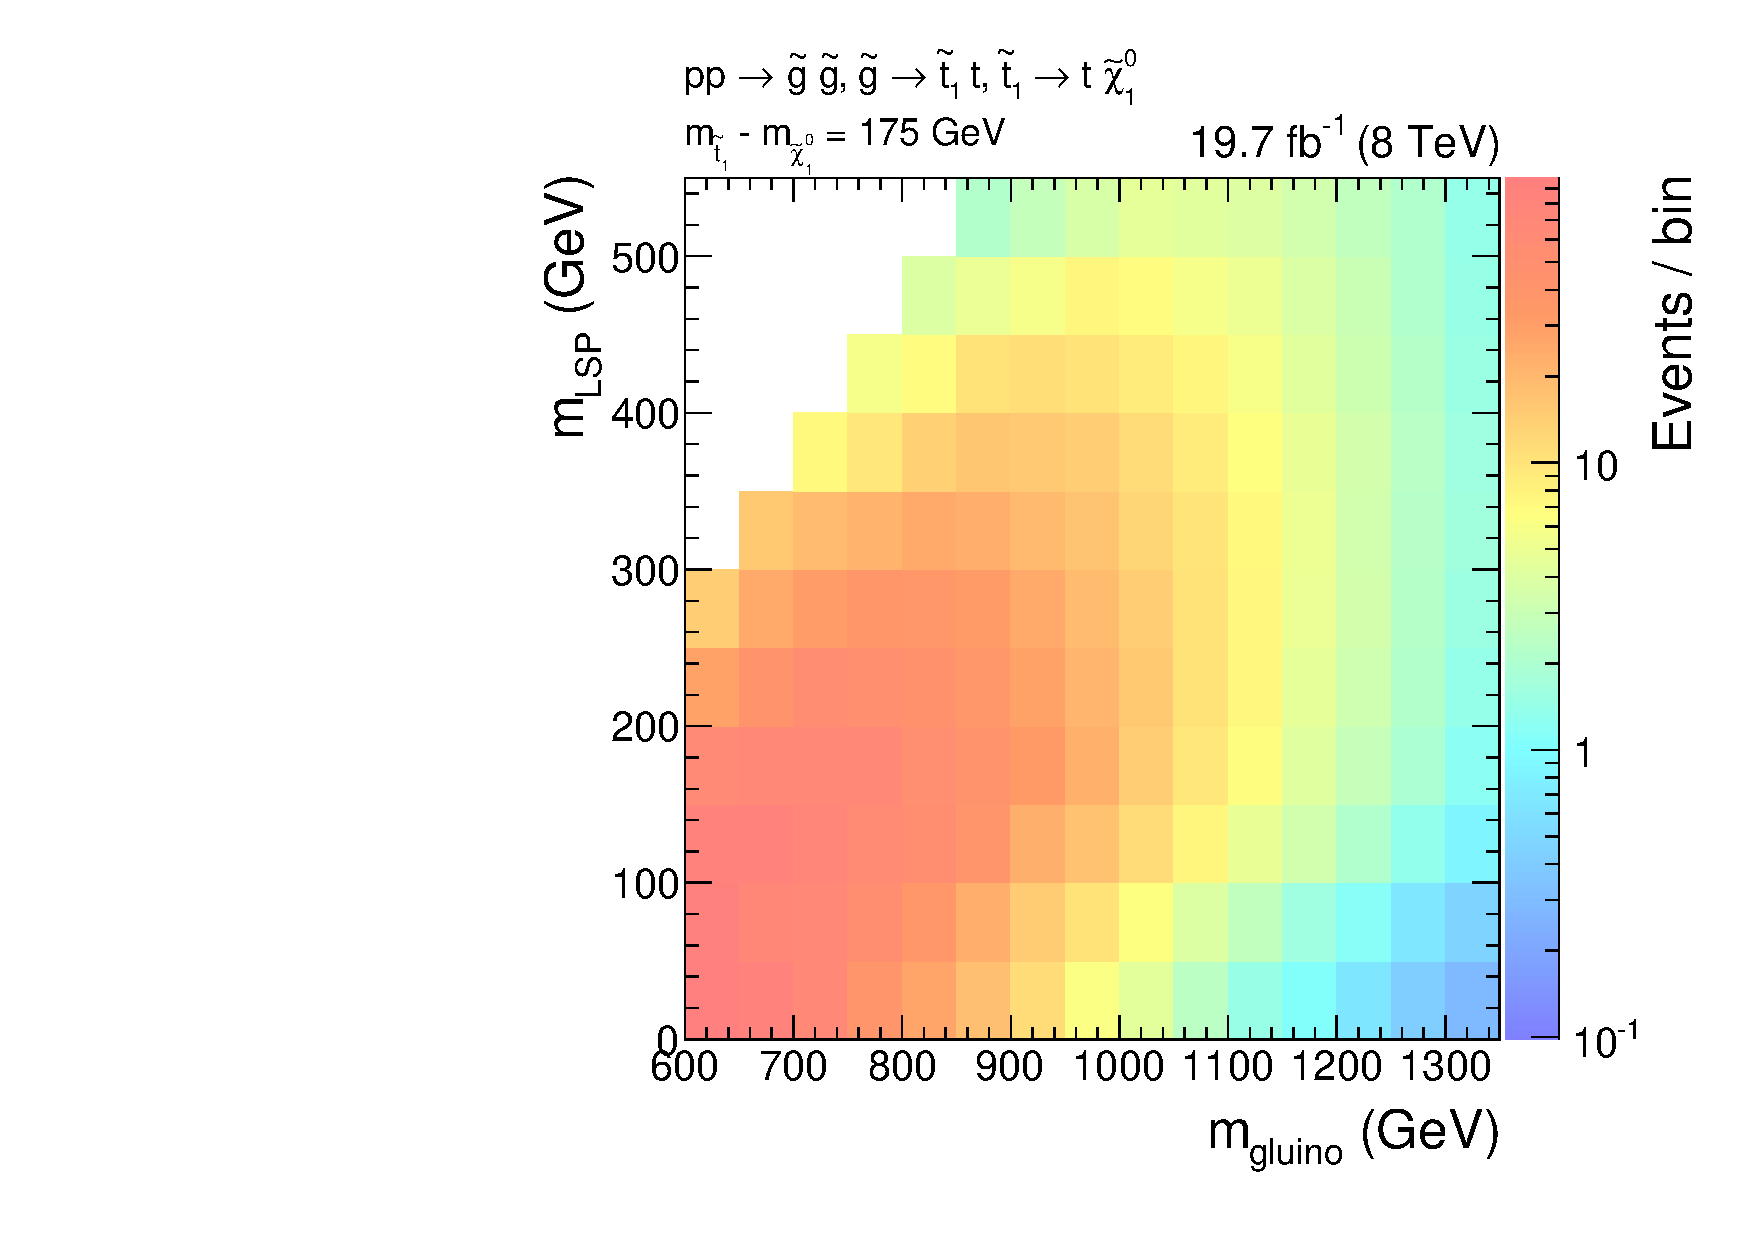
\includegraphics[width=0.3\textwidth]{figures/T1t1t/events_T1t1t_g1Mbg1W0Ll_mdPhig0p5} ~
%  \includegraphics[width=0.3\textwidth]{figures/T1t1t/significance_T1t1t_g1Mbg1W0Ll_mdPhig0p5}
%  \caption{Signal region efficiency, number of events in $19.712\textrm{fb}^{-1}$ and significance
% $\frac{S}{\sqrt{B}}$ for the T1t1t simplified model.
%  \label{fig:eff_T1t1t}}
% \end{figure}
% 
% \begin{figure}[htbp]
%  \centering
%   \includegraphics[width=0.3\textwidth]{figures/T2tt/efficiency_T2tt_g1Mbg1W0Ll_mdPhig0p5} ~
%  \includegraphics[width=0.3\textwidth]{figures/T2tt/events_T2tt_g1Mbg1W0Ll_mdPhig0p5} ~
%  \includegraphics[width=0.3\textwidth]{figures/T2tt/significance_T2tt_g1Mbg1W0Ll_mdPhig0p5}
%  \caption{Signal region efficiency, number of events in $19.712\textrm{fb}^{-1}$ and significance
% $\frac{S}{\sqrt{B}}$ for the T2tt simplified model.
%  \label{fig:eff_T2tt}}
% \end{figure}
